\chapter{Интеграция Экосистемы OSTIS с современными сервисами и информационными ресурсами}
\chapauthortoc{Загорский~А.~Г.\\Таранчук~В.Б.\\Шункевич~Д.В.\\Соловьев~А.~М.\\Коршунов ~Р.~А.\\Савенок~В.~А.}
{\label{chapter_integration}}

\vspace{-7\baselineskip}

\begin{SCn}
\begin{scnrelfromlist}{автор}
	\scnitem{Загорский~А.~С.}
	\scnitem{Таранчук~В.~Б.}
	\scnitem{Шункевич~Д.~В.}
	\scnitem{Соловьев~А.~М.}
	\scnitem{Коршунов~Р.~А.}	
	\scnitem{Савенок~В.~А.}
\end{scnrelfromlist}

\bigskip

\scntext{аннотация}{В главе описываются общие принципы \textit{интеграции}, а также принципы \textit{интеграции} \textit{Экосистемы OSTIS} с разнородными \textit{сервисами} и структурированными \textit{информационными ресурсами}. Также описывается \textit{интеграция} инструментов компьютерной алгебры в \textit{ostis-системы}. Эта глава будет полезна для специалистов в области программной инженерии, искусственного интеллекта и системного анализа, которые заинтересованы в \textit{интеграции} различных \textit{сервисов} и \textit{ресурсов} в \textit{интеллектуальные системы}.}

\bigskip

\begin{scnrelfromlist}{подраздел}
	\scnitem{\ref{sec_integration_common_principles}~\nameref{sec_integration_common_principles}}
	\scnitem{\ref{sec_integration_algebra}~\nameref{sec_integration_algebra}}
\end{scnrelfromlist}

\bigskip

\begin{scnrelfromlist}{ключевое понятие}
	\scnitem{интеграция}
	\scnitem{информационный ресурс}
	\scnitem{сервис}
\end{scnrelfromlist}

\bigskip

\begin{scnrelfromlist}{ключевой знак}
	\scnitem{Экосистема OSTIS}
\end{scnrelfromlist}

\bigskip

\begin{scnrelfromlist}{библиографическая ссылка}
	\scnitem{\scncite{Valdez2019}}
	\scnitem{\scncite{Li2012a}}
	\scnitem{\scncite{Caldarola2015}}
	\scnitem{\scncite{Bork2019}}
	\scnitem{\scncite{Kroshchanka2022}}
	\scnitem{\scncite{RDF}}
	\scnitem{\scncite{R2RML}}
	\scnitem{\scncite{R2RMLIO}}
	\scnitem{\scncite{INFOLAKE}}
	\scnitem{\scncite{Dyakonov2022}}
	\scnitem{\scncite{Aladiev1999}}
	\scnitem{\scncite{Aladiev2011}}
	\scnitem{\scncite{CAS2023}}
	\scnitem{\scncite{CASTypes2023}}
	\scnitem{\scncite{Maxima2023}}
	\scnitem{\scncite{Stahin2008}}
	\scnitem{\scncite{AXIOM2023}}
	\scnitem{\scncite{Dyakonov2022b}}
	\scnitem{\scncite{MATLABVersions2023}}
	\scnitem{\scncite{MATLABLanguage2023}}
	\scnitem{\scncite{MAPLEBooks2023}}
	\scnitem{\scncite{Dyakonov2022c}}
	\scnitem{\scncite{Aladiev2006}}
	\scnitem{\scncite{MAPLEHistory2023}}
	\scnitem{\scncite{Dyakonov2022a}}
	\scnitem{\scncite{WolframBooks2023}}
	\scnitem{\scncite{SRPM2023}}
	\scnitem{\scncite{WolframMath2023}}
	\scnitem{\scncite{WolframAlpha}}
	\scnitem{\scncite{MathematicaHistory2023}}
	\scnitem{\scncite{MathematicaRevision2023}}
	\scnitem{\scncite{Taranchuk2019}}
	\scnitem{\scncite{Taranchuk2019a}}
\end{scnrelfromlist}

\end{SCn}

\section*{Введение в Главу \ref{chapter_integration}}
Важным является не только сама \textit{Экосистема OSTIS} как форма реализации Общества 5.0, но и процесс поэтапного перехода от современной глобальной сети \textit{компьютерных систем} к глобальной сети \textit{ostis-систем}, то есть к \textit{Экосистеме OSTIS}.

\textit{интеграция} современных \textit{сервисов} и \textit{информационных ресурсов} с \textit{Экосистемой OSTIS} является важнейшим элементом для продвижения технологических инноваций в современном мире. Поскольку спрос на эффективные, надежные и доступные системы продолжает расти, очень важно иметь комплексную и интегрированную платформу, способную удовлетворить различные потребности.

\textit{Технология OSTIS} обеспечивает основу для разработки сложных систем и их беспрепятственной \textit{интеграции} c существующими услугами и \textit{ресурсами}. Системы, разработанные в раммках комплексной экосистемы в совокупности предоставляют возможности использовать самый разнообразный функционал: управление информацией, анализ данных, принятие решений, автоматизацию и так далее.

В данной главе рассматривается значение \textit{интеграции} \textit{Экосистемы OSTIS} с современными \textit{сервисами} и \textit{информационными ресурсами}, а также потенциальные преимущества такой \textit{интеграции}. 
Цель данной главы --- дать всесторонний анализ и представить аргументы в пользу внедрения современных систем и \textit{сервисов} в \textit{Экосистему OSTIS}.

\section{Общие принципы интеграции Экосистемы OSTIS с современными сервисами и информационными ресурсами}
{\label{sec_integration_common_principles}}

\begin{SCn}
    
    \begin{scnrelfromlist}{подраздел}
        \scnitem{\ref{sec_integration_services}~\nameref{sec_integration_services}}
        \scnitem{\ref{sec_integration_resources}~\nameref{sec_integration_resources}}
    \end{scnrelfromlist}
    
\end{SCn}

\subsection*{Введение в \ref{sec_integration_common_principles}}

Процесс \textit{интеграции} \textit{Экосистемы OSTIS} с \textit{сервисами} и \textit{информационными ресурсами} требует глубокого понимания базовых принципов \textit{Технологии OSTIS}. 
В этом параграфе рассмотрены общие принципы \textit{интеграции} \textit{Экосистемы OSTIS} с современными \textit{сервисами} и \textit{информационными ресурсами}, как она может быть адаптирована для интеграции с различными \textit{сервисами} и \textit{ресурсами}, включая \textit{базы данных}, \textit{веб-сервисы} и \textit{облачные системы}.

Общие принципы \textit{интеграции} \textit{цифровой экосистемы} с современными \textit{сервисами} и \textit{информационными ресурсами} выглядят следующим образом (см. \scncite{Valdez2019}, \scncite{Li2012a}):
\begin{textitemize}
    \item \textit{стандартизация} и \textit{совместимость}, что достигается путем использования стандартизованных протоколов и форматов обмена данными.
    \item \textit{открытость} и доступность \textit{цифровой экосистемы} для различных участников, что обеспечениватся открытыми и удобными \textit{интерфейсами}.
    \item \textit{безопасность} и конфиденциальность, что достигается путем использования криптографических методов защиты данных и контроля доступа к ресурсам.
    \item \textit{автоматизация} и \textit{масштабируемость}, что позволит обеспечить эффективность и производительность \textit{цифровой экосистемы} при работе с большим количеством \textit{сервисов} и \textit{ресурсов}.
    \item анализ и управление данными, что поможет определить эффективность \textit{интеграции} и улучшить ее в дальнейшем.
\end{textitemize}

Каждый из этих принципов играет важную роль в \textit{интеграции} \textit{цифровой экосистемы} с современными \textit{сервисами} и \textit{информационными ресурсами} и должен быть учтен при разработке и реализации интеграционных решений. Важно отметить, что для успешной \textit{интеграции} необходимо учитывать специфику каждой конкретной системы и ее потребностей. Это требует анализа и понимания всех особенностей и требований, которые могут повлиять на процесс \textit{интеграции}.

В целом, для успешной \textit{интеграции} \textit{цифровой экосистемы} с современными \textit{сервисами} и \textit{информационными ресурсами} необходимо учитывать все указанные принципы и использовать современные технологии, такие как \textit{Технология OSTIS}, которые позволяют реализовать эти принципы в практической работе.

\textit{Технология OSTIS} представляет собой мощный инструмент для разработки и реализации \textit{цифровых экосистем}, которые могут интегрироваться с различными \textit{сервисами} и \textit{информационными ресурсами}. Она обладает рядом преимуществ, таких как использование открытых стандартов и моделей, возможность масштабирования и автоматизации процессов, высокий уровень безопасности и конфиденциальности, а также удобные \textit{интерфейсы} для работы с данными.

\textit{ostis-системы} могут выполнять роль системных интеграторов различных \textit{ресурсов} и \textit{сервисов}, реализованных современными \textit{компьютерными системами}, поскольку \textit{уровень интеллекта} \textit{ostis-систем} позволяет им с любой степенью детализации специфицировать интегрируемые \textit{компьютерные системы} и, следовательно, достаточно адекватно понимать, что знает и/или умеет каждая из них. Также \textit{ostis-системы} способны достаточно качественно координировать деятельность стороннего \textit{ресурса} и \textit{сервиса} и обеспечивать релевантный поиск нужного \textit{ресурса} или \textit{сервиса}.

Кроме того \textit{ostis-системы} могут выполнять роль интеллектуальных help-систем --- помощников и консультантов по вопросам эффективной эксплуатации различных \textit{компьютерных систем} со сложными функциональными возможностями, имеющими \textit{пользовательский интерфейс} с нетривиальной семантикой и использующимися в сложных предметных областях. 
Такие интеллектуальные help-системы можно сделать интеллектуальными посредниками между соответствующими \textit{компьютерными системами} их пользователями.

На первых этапах перехода к Обществу 5.0 нет необходимости преобразовывать в \textit{ostis-системы} все современные системы автоматизации некоторых видов и областей человеческой деятельности. 
Однако, \textit{ostis-системы} должны взять на себя координационно-связующую роль благодаря высокому уровню своей \textit{интероперабельности}. 
\textit{ostis-системы} должны научиться либо выполнять миссию активной интероперабельной надстройки над различными современными средствами автоматизации, либо ставить перед современными средствами автоматизации выполнимые для них задачи, обеспечивая их непосредственное участие в решении сложных комплексных задач и организуя управление взаимодействием различных средств автоматизации в процессе коллективного решения сложных комплексных задач.

\subsection{Принципы интеграции Экосистемы OSTIS с разнородными сервисами}
{\label{sec_integration_services}} 

В контексте интеграции \textit{Экосистемы OSTIS} с разнородными \textit{сервисами}, под \textit{сервисами} понимаются приложения, программы, \textit{веб-сервисы} и другие \textit{информационные системы}, которые предоставляют определенный функционал, механизм преобразования информации в соответствии с заданной функцией. Зачастую такое приложение может предоставить \textit{программный интерфейс}, который можно использовать с определённым форматом входов, которым будут соответствовать определённые форматы выходов.

Под \textit{интеграцией} \textit{Экосистемы OSTIS} с \textit{сервисом} следует понимать возможность использовать функционал \textit{сервиса} для изменения внутреннего состояния \textit{базы знаний} \textit{Экосистемы OSTIS}. 

При \textit{интеграции} \textit{сервисов} в \textit{цифровых экосистемах} возникают ряд проблем, которые могут затруднять процесс \textit{интеграции} и уменьшать эффективность экосистемы (см. \scncite{Valdez2019}, \scncite{Li2012a}). Некоторые из этих проблем могут включать в себя:

\begin{textitemize}
    \item различные форматы данных и протоколы обмена, которые могут привести к ошибкам при \textit{обмене информацией}, что затрудняет взаимодействие между \textit{сервисами};
    \item \textit{несовместимость} версий приложений, что может привести к конфликтам при \textit{обмене информацией};
    \item разные уровни безопасности, что может стать причиной утечки конфиденциальной информации;
    \item отсутствие единой точки управления, что затрудняет мониторинг и управление процессами \textit{интеграции};
    \item отсутствие механизмов для анализа и управления информацией, что затрудняет контроль над процессами \textit{обмена информации}.
\end{textitemize}

Перечисленные проблемы значительно усложняют разработку самих \textit{сервисов} и ведёт к значительному увеличению временных и материальных затрат. Для решения этих проблем при интеграции \textit{цифровых экосистем} с различными \textit{сервисами} и \textit{ресурсами} используются различные подходы и технологии (см \scncite{Caldarola2015}, \scncite{Bork2019}). Некоторые из них могут включать в себя:

\begin{textitemize}
\item использование стандартных протоколов и форматов обмена данных, таких как XML, JSON и другие, что позволяет сделать \textit{обмен информацией} более надежным и универсальным;
\item разработка единой схемы данных и правил доступа, что позволяет сделать \textit{интеграцию} более простой и управляемой;
\item реализация механизмов для автоматической обработки ошибок и конфликтов, что позволяет снизить количество ошибок и улучшить надежность \textit{цифровой экосистемы};
\item использование инструментов и технологий для анализа и управления информацией, таких как системы бизнес-аналитики и управления информацией, что позволяет контролировать процессы \textit{обмена информации} и оптимизировать их работу.
\end{textitemize}


В рамках \textit{Экосистемы OSTIS} выделено несколько уровней \textit{интеграции}, которые позволяют взаимодействовать с различными \textit{информационными ресурсами} и \textit{сервисами}. 

Полная \textit{интеграция} предполагает исполнение функции \textit{сервиса} на платформонезависимом уровне, где вся программа исполняется в самой \textit{базе знаний} \textit{Экосистемы OSTIS}. То есть, задача интеграции такого \textit{сервиса} сводится к выделению алогиртма обработки графовой конструкции и его реализации в рамках \textit{базы знаний}. В результате такой полной интеграции надобность использовать сторонний \textit{сервис} отпадает. 

Частичная \textit{интеграция} предполагает реализацию взаимодействия и изменения состояния \textit{базы знаний} \textit{Экосистемы OSTIS} на этапах исполнения функции \textit{сервиса}. Степень глубины \textit{интеграции} может различаться, в некоторых случаях \textit{сервис} может обращаться к \textit{базе знаний} для получения дополнительной информации или для записи промежуточных результатов. 

В простейшем случае изменение \textit{базы знаний} \textit{Экосистемы OSTIS} может происходить единожды, после получения результата отработки функции \textit{сервиса}. На основе такого принципа можно выделить специальные \textit{sc-агенты}, использующие сторонний \textit{сервис}. 

Для обеспечения \textit{интеграции} функционального \textit{сервиса} необходимо выполнение следующих минимальных требований:
\begin{textitemize}
    \item спецификация входной конструкции в \textit{базе знаний} системы: определение структуры в \textit{базе знаний} системы, которая будет преобразовываться в формат данных, совместимый с \textit{сервисом};
    \item спецификация выходной конструкции в \textit{базе знаний} системы: определение структуры в \textit{базе знаний} системы, которая будет формироваться из исходной структуры впоследствии преобразования данных \textit{сервиса} в знания;
    \item реализация \textit{sc-агента}, который преобразует конструкцию \textit{базы знаний} в формат, который может быть использован в \textit{сервисе}, а также погружать результаты работы \textit{сервиса} обратно в \textit{базу знаний} системы в соответствии со спецификацией.
\end{textitemize}

Удовлетворение данных требований позволит обеспечить эффективную \textit{интеграцию} функционального \textit{сервиса}, что, в свою очередь, позволит использовать данные и функциональность \textit{сервиса} в различных \textit{ostis-системах}. Задача формирования спецификации рассмотрена в \ref{sec_kb_design_methods}~\nameref{sec_kb_design_methods}.

Обобщенный алгоритм \textit{sc-агента}, использующего сторонний \textit{сервис} для \textit{интеграции} функциональных возможностей, может быть описан следующим образом:

\begin{textitemize}
    \item извлечение из \textit{базы знаний} необходимых структур знаний, соответствующих требованиям функционального \textit{сервиса};
    \item преобразование извлечённых знаний в формат, необходимый для подачи на вход функциональному \textit{сервису};
    \item отправка запроса на функциональный \textit{сервис} и ожидание его ответа;
    \item формирование структур знаний на основе полученных данных от функционального \textit{сервиса};
    \item погружение новых структур знаний в \textit{базу знаний} \textit{интеллектуальной системы}, с целью обеспечения их дальнейшей использования.
\end{textitemize}

Следует учесть, что при \textit{интеграции} функциональных \textit{сервисов}, возможно потребуется проводить дополнительную обработку и преобразование данных, например, для обеспечения их \textit{совместимости} с форматами данных, или для обеспечения безопасности передачи и хранения данных.

Таким образом, внедрение возможности использования стороннего \textit{сервиса} в \textit{Экосистеме OSTIS} предполагает выполнение следующих шагов:
\begin{textitemize}
    \item анализ требований к интегрируемому \textit{сервису}, определение необходимого функционала, форматов входных и выходных данных, и других характеристик сервиса.
    \item разработка спецификации \textit{интеграции}, которая будет определять форматы данных и правила взаимодействия между \textit{базой знаний} \textit{Экосистемы OSTIS} и сторонним \textit{сервисом};
    \item разработка \textit{sc-агента}, который будет обеспечивать взаимодействие между \textit{базой знаний} и сторонним \textit{сервисом} в соответствии со спецификацией \textit{интеграции};
    \item тестирование и отладка;
    \item внедрение в \textit{Экосистему OSTIS}, что позволит использовать возможности интегрированного стороннего \textit{сервиса} в различных \textit{ostis-системах}.
\end{textitemize}

Для подключения \textit{sc-агента} используются различные подходы, один из которых заключается в подключении \textit{sc-агента} в рамках уже существующей, основной \textit{ostis-системы}. С точки зрения масштабируемости реализации такого подхода следует отметить \textit{монолитную архитектуру} получаемой \textit{ostis-системы}, что позволяет упростить процесс внедрения новых \textit{сервисов} и \textit{sc-агентов} в \textit{ostis-систему}.

Преимуществом такого подхода является более простое и удобное внедрение новых \textit{сервисов} и \textit{sc-агентов} в \textit{ostis-систему}, а также упрощение процесса управления зависимостями. Использование реализации ostis-системы с \textit{монолитной архитектурой} может быть применено в случаях, когда функциональный \textit{сервис} не нуждается в частой модификации и обладает достаточно простой структурой. Кроме того, \textit{монолитная архитектура} может быть более удобна в случаях, когда обращение к \textit{сервису} происходит через внутреннюю сеть и требует низкой задержки и высокой производительности. Так могут быть интегрированы и \textit{сервисы} получения знаний из внешних источников (получение прогноза погоды, обработка статистической информации, и так далее), и функциональные \textit{сервисы} (обработка аудиоинформации и погружение результатов обработки в \textit{базу знаний}, получение синтаксического анализа предложения). 

Альтернативным вариантом внедрения является реализация отдельной \textit{ostis-системы}, в рамках которой будет интегрирована функция \textit{сервиса}. Это позволяет перейти к использованию \textit{микросервисной архитектуры}, что характеризуется распределенным взаимодействием \textit{ostis-систем}.

Преимуществами такого подхода является большая \textit{гибкость} и возможность \textit{масштабирования}. Подход характеризуется высокой степенью распределённости, децентрализованности и доступности нового функционала. Система выходит за рамки технических ограничений, функционал может быть распределён на различном аппаратном обеспечении. Полученный функционал может быть использован различными \textit{ostis-системами} в рамках \textit{Экосистемы OSTIS} для достижения своих целей. Минусами такой системы является сложность разработки, а также увеличение временных затрат на общение систем друг с другом по сетевым протоколам. 

\textit{микросервисную архитектуру} ostis-систем предпочтительно использовать в случаях, когда функциональный \textit{сервис} обладает сложной структурой, а также в случаях, когда требуется масштабирование и гибкость всей системы. В качестве примера можно привести \textit{сервис}, который взаимодействует с внешними источниками данных и может быть подвержен частым изменениям.  Примерами \textit{интеграции} на основе \textit{микросервисной архитектуры} могут служить \textit{сервисы} считывания эмоционального состояния пользователя, естественно-языковая обработка, задачи классификации и идентификации, и так далее.

Таким образом, выбор подхода к \textit{интеграции} функциональных \textit{сервисов} зависит от конкретных требований и условий проекта. Использование \textit{Технологии OSTIS} позволяет создавать гибкие и эффективные системы, которые могут быть адаптированы под различные потребности и требования пользователей.

\subsection{Принципы интеграции Экосистемы OSTIS со структурированными информационными ресурсами}
{\label{sec_integration_resources}} 

\begin{SCn}
\bigskip

\begin{scnrelfromlist}{библиографическая ссылка}
    \scnitem{\scncite{RDF}}
    \scnitem{\scncite{R2RML}}
    \scnitem{\scncite{R2RMLIO}}
    \scnitem{\scncite{INFOLAKE}}
\end{scnrelfromlist}
\end{SCn}

Существует несколько причин, по которым следует интегрировать интеллектуальную систему с информационными источниками:
\begin{textitemize}
    \item Обеспечение полноты и точности данных: Интеллектуальная система создается для обработки больших объемов данных и принятия решений на их основе. Информационные источники являются основой для этих данных, и интеграция системы с ними гарантирует полноту и точность данных.
    \item Уменьшение времени и усиление эффективности работы: Интеграция информационных источников в интеллектуальную систему обеспечивает быстрый и удобный доступ к нужной информации. Это уменьшает время на поиск и обработку данных, что повышает эффективность работы системы и уменьшает количество ошибок.
    \item Расширение возможностей системы: Информационные источники обладают большим количеством данных, которые могут быть полезны для работы интеллектуальной системы. Интеграция системы с различными источниками расширяет возможности системы и позволяет ей повысить качество работы.
    \item Повышение надежности: Разнообразные источники данных обеспечивают резервирование и возможность сравнения, что позволяет интеллектуальной системе работать более надежно и безопасно в случае сбоя одного или нескольких источников.
    \item Улучшение качества прогнозирования: Интеграция информационных источников с интеллектуальной системой способствует улучшению качества прогнозирования, так как позволяет объединять данные из различных источников и анализировать их вместе для получения более точных результатов.
\end{textitemize}

Существует большое количество информационных источников, из которых можно получать информацию. Основными можно назвать следующие:
\begin{textitemize}
    \item Интернет --- сайты, блоги, форумы, социальные сети, новостные порталы и другие ресурсы в сети.
    \item Книги и учебники --- доступные в библиотеках, книжных магазинах или в электронном формате.
    \item СМИ --- телевизионные программы, радио, газеты, журналы и другие источники новостей.
    \item Официальные документы и отчеты --- включая законы, правительственные статистические данные, отчеты об исследованиях и другие официальные документы.
\end{textitemize}

Принципы интеграции \textit{Экосистемы OSTIS} со структурированными информационными ресурсами основаны на пополнении базы знаний системы новыми знаниями. Один из востребованных подходов в этом направлении --- интеграция с ресурсами на основе RDF (Resource Description Framework, см. \scncite{RDF}), который является моделью данных, предложенной консорциумом W3C.

Для успешной интеграции структурированных информационных ресурсов в Экосистему OSTIS, важно уделить должное внимание пониманию и применению принципов RDF-модели, поскольку они играют ключевую роль в организации связей между различными ресурсами. RDF используется для описания ресурсов в сети Интернет, и является основой для построения семантических веб-приложений, таких как Linked Open Data.

Основная структура абстрактного синтаксиса RDF --- это тройка, состоящая из субъекта, предиката и объекта. Набор таких троек называется графом RDF. Граф RDF может быть визуализирован как диаграмма узла и направленной дуги, в которой каждая тройка представлена как связь ``узел --- дуга --- узел''.

Графы RDF атемпоральны, т.е. представляют собой статические снимки информации. Однако графы RDF могут выражать информацию о событиях и временных аспектах других сущностей, учитывая соответствующие термины из словаря. Поскольку графы RDF определены как математические наборы, добавление или удаление троек из графа RDF дает другой граф RDF.

Узел может иметь следующий тип:
\begin{textitemize}
    \item IRI. Представляет собой короткую последовательность символов, идентифицирующую абстрактный или физический ресурс на любом языке мира. IRI представляе собой обобщение URI;
    \item Литерал. Представляя собой структуру, состоящую из лексической формы (UNICODE-строка) и типа данных;
    \item Пустой узел. Представляет собой локальный идентификатор, который используются в некоторых конкретных синтаксисах RDF или реализациях хранилища RDF.
\end{textitemize}

RDF поддерживает основные типы данных, такие как строковый (string), логический (boolean), числовые (integer, double, float и др.), временные и некоторые другие.

В RDF существует такое понятие, как словарь RDF. Он представляет собой совокупность IRI, ссылающихся на другие графы с классами, литералами и др. Часто группа IRI может начинаться с одинакового префикса.

RDF нашел широкое применение. Так, например, RDF используется в оформлении \textit{баз знаний} в рамках различных проектов во множестве институтов, университетов и иных организаций. Поисковые системы предлагают веб-мастерам использовать RDF и аналогичные языки разметки страниц для повышения информативности ссылок на их сайты в результатах поиска. Социальные сети, с подачи Facebook, предлагают веб-мастерам использовать RDF для описания свойств страниц, так же позволяющих красиво оформить ссылку на неё в записи пользователя социальной сети.

В ходе анализа были выявлены следующие подходы к интеграции информационных ресурсов на основе RDF с другими системами:
\begin{textitemize}
    \item R2RML (см. \scncite{R2RML}) --- это стандарт W3C для выражения настраиваемых отображений из реляционных БД в RDF. Такие отображения предоставляют возможность просматривать существующие реляционные данные в модели данных RDF, выраженные в структуре и целевом словаре по выбору автора сопоставления;
    \item R2RML.io (см. \scncite{R2RMLIO}) --- это open-source проект, разрабатываемый с 2013 года. Данная технология предназначена для генерации базы знаний на основе данных из полуструктурированных источников;
    \item ``Озеро данных'' (см. \scncite{INFOLAKE}) --- это централизованное хранилище, которое позволяет хранить все структурированные и неструктурированные данные в любом масштабе. ``Семантическое озеро данных'' --- это особая форма озер данных, в которых верхний семантический слой обогащает и связывает данные семантически. Семантический уровень преодолевает разрозненность данных и обеспечивает семантический поиск по всем данным.
\end{textitemize}

Интеграция ostis-систем с внешними информационными ресурсами удобна по многим причинам. Технология OSTIS изначально предлагает инструменты для описания синтаксиса и семантики внешних языков (см. \textit{Главу \ref{chapter_ext_lang} \nameref{chapter_ext_lang}}). Данный инструментарий позволяет сократить время разработки в несколько раз. Также из достоинств можно выделить:
\begin{textitemize}
    \item способность осуществлять интеграцию знаний в своей памяти на высоком уровне;
    \item возможность интегрировать различные виды знаний;
    \item возможность интегрировать различные модели решения задач.
\end{textitemize}

Для интеграции информационного ресурса на основе RDF в Экосистему OSTIS был реализован соответствующий \textit{абстрактный sc-агент}. Его работу можно разбить на следующие этапы:
\begin{textitemize}
    \item интеграция с использованием готовых правил;
    \item интеграция с сохранением исходной схемы;
    \item дополнительные преобразования.
\end{textitemize}

\textbf{Интеграция с использованием готовых правил}

На этом этапе ко всем сгенерированным тройкам применяются готовые правила интеграции, хранящиеся в \textit{базе знаний}. Создание и применение подобных правил необходимо в ситуациях, когда способ представления конкретного знания во внешнем информационном ресурсе по какой-то причине не соответствует представлению аналогичного знания в ostis-системе.

\textbf{Интеграция с сохранением исходной схемы}

На данном этапе оставшиеся тройки будут преобразованы с сохранением той структуры отношения, в которой находились участвовавшие в нем сущности. Это значит, что порядок элементов в итоговой конструкции будет аналогичен порядку сущностей в исходной.

\textbf{Дополнительные преобразования}

На данном этапе проходят оставшиеся интеграционные преобразования, которым не нашлось места в предыдущих пунктах, но которые необходимы для завершения процесса интеграции.

Для выгрузки информации из \textit{базы знаний} в какой-либо внешний формат можно использовать те же правила, что и для загрузки, так как в основном они представляют собой утверждения об \textit{эквиваленции}. То есть изначально производится поиск необходимых конструкций, затем они к ним применяется соответствующее правило, и, в результате получается множество троек. В дальнейшем данные тройки преобразуются в необходимый формат.
\newpage

\section{Интеграция инструментов компьютерной алгебры в приложения OSTIS}
{\label{sec_integration_algebra}} 

\begin{SCn}

\bigskip

\begin{scnrelfromlist}{ключевое понятие}
	\scnitem{компьютерная алгебра}
	\scnitem{система компьютерной математики}
	\scnitem{система компьютерной алгебры}
	\scnitem{системы для численных вычислений}
\end{scnrelfromlist}

\bigskip

\begin{scnrelfromlist}{ключевой знак}
	\scnitem{Maxima}
	\scnitem{MATLAB}
	\scnitem{Mathematica}
	\scnitem{Mapple}
	\scnitem{Wolfram}
	\scnitem{Wolfram Mathematica}
	\scnitem{Wolfram Alpha}
	\scnitem{Wolfram Language}
\end{scnrelfromlist}

\bigskip

\begin{scnrelfromlist}{ключевое знание}
	\scnitem{Способы интеграции систем компьютерной алгебры с Экосистемой OSTIS}
	\scnitem{Принципы интеграции систем компьютерной алгебры с Экосистемой OSTIS}
\end{scnrelfromlist}

\bigskip

\begin{scnrelfromlist}{библиографическая ссылка}
	\scnitem{\scncite{Dyakonov2022}}
	\scnitem{\scncite{Aladiev1999}}
	\scnitem{\scncite{Aladiev2011}}
	\scnitem{\scncite{CAS2023}}
	\scnitem{\scncite{CASTypes2023}}
	\scnitem{\scncite{Maxima2023}}
	\scnitem{\scncite{Stahin2008}}
	\scnitem{\scncite{AXIOM2023}}
	\scnitem{\scncite{Dyakonov2022b}}
	\scnitem{\scncite{MATLABVersions2023}}
	\scnitem{\scncite{MATLABLanguage2023}}
	\scnitem{\scncite{Dyakonov2022с}}
	\scnitem{\scncite{Aladiev2006}}
	\scnitem{\scncite{MAPLEBooks2023}}
	\scnitem{\scncite{MAPLEHistory2023}}
	\scnitem{\scncite{MathematicaHistory2023}}
	\scnitem{\scncite{MathematicaRevision2023}}
	\scnitem{\scncite{Dyakonov2022a}}
	\scnitem{\scncite{WolframBooks2023}}
	\scnitem{\scncite{WolframMath2023}}
	\scnitem{\scncite{Taranchuk2019}}
	\scnitem{\scncite{Taranchuk2019a}}
	\scnitem{\scncite{SRPM2023}}
	\scnitem{\scncite{WolframAlpha}}
\end{scnrelfromlist}

\bigskip

\begin{scnrelfromlist}{подраздел}
	\scnitem{\ref{subsec_cas_principles}~\nameref{subsec_cas_principles}}
	\scnitem{\ref{subsec_cas_survey}~\nameref{subsec_cas_survey}}
	\scnitem{\ref{subsec_cas_intergation}~\nameref{subsec_cas_intergation}}
\end{scnrelfromlist}

\end{SCn}

\subsection*{Введение в \ref{sec_integration_algebra}}

В середине XX века на стыке математики и информатики возникло и интенсивно развивается фундаментальное научное направление --- \textbf{\textit{компьютерная алгебра}}, наука об эффективных алгоритмах вычислений математических объектов. Синонимами термина \textit{``компьютерная алгебра''} являются: \textit{``символьные вычисления''}, \textit{``аналитические вычисления'}', \textit{``аналитические преобразования''}, а иногда и \textit{``формальные вычисления''}. Направление ``компьютерная алгебра'' представлено теорией, технологиями, программными средствами. К прикладным результатам относят разработанные алгоритмы и программное обеспечение для решения с помощью компьютера задач, в которых исходные данные и результаты имеют вид математических выражений, формул. Основным продуктом компьютерной алгебры стали программные \textit{системы компьютерной алгебры} --- \textbf{\textit{с.к.а.}} (англ. Computer Algebra System, CAS). 

Круг математических задач, которые можно решить с помощью \textit{с.к.а.}, непрерывно расширяется. Значительные усилия исследователей направлены на разработку алгоритмов вычисления топологических инвариантов многообразий, узлов, алгебраических кривых, когомологий различных математических объектов, арифметических инвариантов колец целых элементов в полях алгебраических чисел. Другое направление современных исследований --- квантовые алгоритмы, имеющие иногда полиномиальную сложность, тогда как существующие классические алгоритмы имеют экспоненциальную.

Исследования и разработки теоретических основ и технологий реализации методов и программных реализаций инструментов компьютерной алгебры продолжаются. Термины, определения, названия в описаниях функций и инструментов этих систем также претерпевают изменения, некоторые формулировки, ранее приводимые в отдельных руководствах, обзорах возможностей инструментария не только уточняются, но и изменяются. Это нормально для новых научных направлений и технологий. Читатель не должен удивляться, если в других источниках встретит иные формулировки, термины.

Не следует отождествлять \textit{системы компьютерной алгебры} и \textit{системы компьютерной математики} (\textbf{\textit{с.к.м.}}), которые в ряде изданий условно делятся на две категории: \textit{системы компьютерной алгебры} и \textit{системы для численных вычислений}. Обычно к \textit{с.к.м.} относят:
\begin{textitemize}
	\item табличные процессоры, например, \textit{Microsoft Excel}, \textit{Lotus Symphony Spreadsheets}, \textit{Gnumeric, OpenOffice.org Calc};
	\item системы для статистических расчетов, например, \textit{STATISTICA}, \textit{PASW Statistics} (первоначальное название \textit{SPSS Statistics});
	\item системы для моделирования, анализа и принятия решений, например, GPSS, AnyLogic, DSS;
	\item системы компьютерной алгебры;
	\item универсальные математические системы.
\end{textitemize}

Если с выделением в отдельные группы первых трех из перечисленных \textit{с.к.м.} есть согласие большинства авторов, то отнесение в отдельную группу универсальных математических систем прослеживается относительно редко. Основные \textit{с.к.а.} в контексте численных и аналитических вычислений большинством авторов считаются универсальными системами.

При развитии технологий на первом месте в разработке и модернизации \textit{и.к.с.} должны быть решения, реализации интеграции таких систем и средств \textit{систем компьютерной алгебры}. 
Важно превращение современного многообразия инструментальных средств (frameworks) разработки различных компонентов \textit{и.к.с.} в единую технологию комплексного проектирования и поддержки полного жизненного цикла этих систем, гарантирующую совместимость всех разрабатываемых компонентов, а также совместимость самих \textit{и.к.с.} как самостоятельных субъектов, взаимодействующих между собой в рамках комплексных систем автоматизации сложных видов коллективной человеческой деятельности. Необходима конвергенция и унификация интеллектуальных компьютерных систем нового поколения и их компонентов (см. \textit{Главу \ref{chap_intro}~\nameref{chap_intro}}, \textit{Главу \ref{chapter_new_generation_systems}~\nameref{chapter_new_generation_systems}}, \textit{Главу \ref{chapter_ostis_tech}~\nameref{chapter_ostis_tech}}). 
При этом, под конвергентными решениями, в основном, подразумеваются оптимизированные комплексы, содержащие в себе все необходимое для решения задач Искусственного интеллекта, организованные или сконфигурированные для эффективного использования информационных ресурсов, для упрощения процессов внедрения; в том числе, должны обеспечиваться возможности решения определенных задач с требованиями оптимизации и достижения максимальной производительности, и во всех реализациях --- оптимизированные для простоты использования. Перечисленное в полной мере относится к \textit{Экосистеме OSTIS}. 

Подобные проблемы решаются и при разработке, совершенствовании, систематическом обновлении содержания и расширения возможностей систем компьютерной алгебры. Таким образом интеграция \textit{с.к.а.} и \textit{Экосистемы OSTIS} является важной и актуальной задачей.

Одним из вариантов взаимодействия \textit{Экосистемы OSTIS} и \textit{с.к.а.} могут быть подходы, аналогичные реализуемым в рамках интеграции в ostis-системы искусственных нейронных сетей (см. \textit{Главу \ref{chapter_ann}~\nameref{chapter_ann}}). Можно рассматривать следующие методические и технические решения:
\begin{textitemize}
	\item Интеграция по принципу "черного ящика"{}, когда в \textit{базе знаний} \textit{ostis-системы} присутствует спецификация используемой функции ядра системы компьютерной алгебры, а также спецификация способа вызова данной функции (например, указание через какой программный интерфейс осуществляется взаимодействие с данной внешней системой). Такой вариант интеграции является наиболее простым в плане реализации и в целом обладает перечисленными выше достоинствами. В то же время, данный вариант обладает и недостатком, связанным с тем, что \textit{ostis-система} не содержит средств анализа и объяснения того, как был выполнен конкретный шаг решения задачи, реализуемый используемой функцией \textit{с.к.а.}
	\item Более тесная интеграция, при которой конкретная функция по-прежнему остается частью сторонней \textit{с.к.а.}, когда в \textit{базу знаний} \textit{ostis-системы} погружается не просто результат ее выполнения, а и всевозможная его спецификация, например, объяснение хода решения задачи, указание конкретных алгоритмов и формул, которые могут быть задействованы в решении, описание возможных альтернативных вариантов решения, оценка эффективности решения и так далее. В данном варианте интеграции \textit{ostis-система} получает больше возможностей по анализу и объяснению хода решения задачи. (Следует отметить, что конкретно в \textit{с.к.а.} \textit{Wolfram Mathematica} уже присутствуют подробные пояснения хода решения задачи и допустим режим пошагового выполнения).
	\item Полная интеграция, при которой осуществляется трансляция используемых функций системы компьютерной алгебры с внутреннего языка этой системы в \textit{ostis-систему}. Данный вариант является наиболее трудоемким и сложным с точки зрения актуализации реализации возможностей систем компьютерной алгебры в соответствующих \textit{ostis-системах} с учетом их постоянного развития. В то же время такой вариант интеграции по сравнению в двумя предыдущими обладает важным достоинством --- он обеспечивает платформенную независимость полученного решения и позволяет использовать при решении конкретной задачи все достоинства предлагаемых в рамках \textit{Технологии OSTIS} подходов, в частности, возможность многопользовательской, параллельной обработки знаний и возможность оптимизации плана решения задачи или его фрагментов непосредственно в ходе решения.
\end{textitemize}

С прикладной точки зрения на данном этапе развития и применения \textit{Экосистемы OSTIS} представляется целесообразной интеграция в едином комплексе возможностей \textit{систем компьютерной алгебры} (\textit{с.к.а.}) и построенных в рамках \textit{Экосистемы OSTIS} интеллектуальных обучающих систем (см. \textit{Главу \ref{chapter_learning_systems}~\nameref{chapter_learning_systems}}), что обусловлено содержанием \textit{систем компьютерной алгебры}, которые обладают несомненным преимуществом и широкими возможностями при решении актуальных для обучающих систем задач практически по всем естественно-научным и техническим дисциплинам, предполагающим использование сложного математического аппарата.

С другой стороны, несмотря на популярность тематики, связанной с автоматизацией и интеллектуализацией образовательной деятельности по естественно-научным дисциплинам и разработкой соответствующих компьютерных систем, на данный момент на рынке практически отсутствуют апробированные \myuline{интеллектуальные} обучающие системы, способные \myuline{самостоятельно генерировать} и решать различные задачи, а также \myuline{проверять корректность решения} задачи пользователем. В качестве прототипов можно привести отдельные системы, в которых решаются нетривиальные задачи, например, по геометрии [https://geometry.allenai.org/, https://mathpix.com/handwriting-recognition ] и теории графов [https://graphonline.ru/]. В то же время следует отметить, что в упомянутых системах нет как таковой "интеллектуальности"{} (по факту заложен только конкретный набор действий, в самих приложениях задачи не генерируются), нет средств проверки решений, имеющих даже незначительные отклонения правил оформления.

Подход к решению задач интеллектуализации образовательной деятельности, основанный на интеграции ostis-систем и систем компьютерной алгебры, обладает рядом преимуществ:
\begin{textitemize}
	\item При разработке \textit{ostis-систем} исключается необходимость программировать многие функции, которые уже реализованы, оттестированы и апробированы в \textit{с.к.а.} Это принципиально, так как системы компьютерной алгебры разрабатываются высококвалифицированными специалистами в соответствующих областях, реализация аналогичных функций в ostis-системах может потребовать значительных финансовых и временных затрат.
	\item Конкретная \textit{ostis-система}, использующая отдельные функции \textit{с.к.а.}, благодаря подходу к разработке гибридных \textit{решателей задач} в \textit{Технологии OSTIS} (см. \textit{Главу \ref{chapter_situation_management}~\nameref{chapter_situation_management}}) получает возможность \myuline{самостоятельно} планировать ход решения задач при условии, что некоторые его этапы будут реализованы при помощи присоединяемых функций. С точки зрения подхода, предлагаемого в рамках \textit{Технологии OSTIS}, каждая функция системы компьютерной алгебры становится \textit{методом} решения задач некоторого класса. Этот класс задач описывается в \textit{базе знаний} \textit{ostis-системы} и позволяет ей при решении конкретной задачи самостоятельно делать вывод о целесообразности применения той или иной функции \textit{с.к.а.} Такая интеграция с \textit{ostis-системами} позволит устранить сформулированный ранее возможный недостаток \textit{систем компьютерной алгебры} (определяется тем, какие \textit{с.к.а.} используются --- отдельно поясняется ниже в обзоре систем компьютерной математики, условий их применения и доступа к отдельным компонентам).
\end{textitemize}

Особо отметим, что обозначенные варианты интеграции не исключают друг друга и могут комбинироваться. Кроме того, углубление интеграции может осуществляться поэтапно с учетом перечисленных достоинств и недостатков, а также с учетом актуальности использования тех или иных функций систем компьютерной алгебры при решении конкретных задач в рамках \textit{Экосистемы OSTIS} и соответствующих \textit{ostis-систем}.

Поэтапная интеграция \textit{с.к.а.} c \textit{Экосистемой OSTIS} предполагает, как минимум, описание спецификации основных функций выбранной системы компьютерной алгебры средствами \textit{Технологии OSTIS}, другими словами --- разработку онтологии внешних функций. В случае с системами семейства \textit{Wolfram Mathematica} процесс разработки такой онтологии может быть автоматизирован благодаря наличию формального языка \textit{Wolfram Language} и хорошей документированности функций системы.

Обобщая изложенное, констатируем --- интеграция обучающих систем, разрабатываемых на базе \textit{Технологии OSTIS}, и систем компьютерной алгебры позволит создавать системы, обладающие высоким уровнем интеллекта, в более сжатые сроки, причем, с использованием тщательно отработанных (математически, алгоритмически) и многократно апробированных инструментов.

\subsection{Назначение, принципы работы, классификация, структура и основные функциональные возможности систем компьютерной алгебры}
\label{subsec_cas_principles}

Основное назначение \textit{с.к.а.} --- работа с математическими выражениями в символьной форме. Базовые типы данных \textit{с.к.а.}: числа и математические выражения. Числа: короткие и длинные целые (одинарной и кратной точности), рациональные, комплексные, алгебраические числа. Алгебраическое число задается своим минимальным многочленом, а иногда для его задания требуется указать интервал на прямой или область в комплексной плоскости, где содержится единственный корень данного многочлена. Математические выражения: арифметика, функции, уравнения, производные, интегралы, векторы, матрицы, тензоры. Кроме того, в компьютерной алгебре рассматриваются такие объекты, как: функциональные, дифференциальные поля, допускающие показательные, логарифмические, тригонометрические функции; матричные кольца и другие. Перечислим основные отличительные признаки систем компьютерной алгебры (см. \scncite{Dyakonov2022}, \scncite{Aladiev1999}, \scncite{Aladiev2011}, \scncite{CAS2023}).

\textbf{с.к.а. работают следующим образом}:
\begin{textitemize}
	\item математические объекты (алгебраические выражения, ряды, уравнения, векторы, матрицы и др.) и указания, что с ними делать, задаются пользователем на входном языке системы в виде символьных выражений;
	\item интерпретатор анализирует и переводит символьные выражения во внутреннее представление;;
	\item символьный процессор системы выполняет требуемые преобразования или вычисления и выдает ответ в математической нотации.
\end{textitemize}
Алгоритмы внутренних преобразований имеют алгебраическую природу, что и отражено в названии систем --- системы компьютерной алгебры.

\textbf{Содержание техники символьных вычислений}:
\begin{textitemize}
	\item внутреннее представление математического выражения в системе символьных вычислений --- синтаксическое дерево (список списков);
	\item суть символьных вычислений (аналитических преобразований) --- переписывание терма с помощью последовательного применения правил из определенного пользователем или системой списка;
	\item преобразование из внешнего представления во внутреннее и обратно обеспечивается дополнительными инструментальными средствами.
\end{textitemize}

Далеко не каждая математическая задача имеет определяемое существующими математическими формализмами аналитическое решение; есть алгоритмически неразрешимые задачи; в исследованиях проблемы оценки трудоемкости алгоритмов алгоритмически разрешимых задач при наличии принципиальных достижений остается значительное число вопросов. Специалисты в областях прикладной и компьютерной математики единодушны во мнении, что много практически важных задач и не могут быть формализованы настолько, чтобы решаться аналитически, в лучшем случае они могут решаться только численными методами.

Достаточно полный перечень с указанием функциональности систем символьных вычислений и платформ, на которых эксплуатируются, можно найти в (см. \scncite{CAS2023}). Классификационными признаками \textit{с.к.а.} являются: функциональное назначение, тип архитектуры, средства реализации, области применения, интегральные оценки качества. Отметим несколько наиболее часто упоминаемых классов.

\textbf{с.к.а. общего назначения и специализированные}. Наиболее известные системы из первой группы (обеспечивают решение задач для большинства основных разделов символьной математики): \textit{Derive}, \textit{Mathematica}, \textit{Maple}, \textit{Macsyma} и ее потомок \textit{Maxima}, \textit{Scratchpad} и ее потомок \textit{Axiom}, \textit{Reduce}, \textit{MuPAD}, \textit{Sage}, \textit{SMath Studio}, \textit{Yacas}, \textit{Scientific WorkPlace}, \textit{Kalamaris}. Системы для решения задач одного или нескольких смежных разделов символьной математики --- это специализированные с.к.а. Примерами таковых являются: \textit{GAP} (теория групп), \textit{Cadabra} (тензорная алгебра), \textit{KANT} (алгебра и теория чисел), \textit{Singular} (полиномиальные вычисления с акцентом на нужды коммутативной алгебры, алгебраическая геометрия), \textit{Calc3D} (для работы с 3D матрицами, векторами, комплексными числами), \textit{GRTensorII} (дифференциальная геометрия).

\textbf{Классы с.к.а. по типу архитектуры}. В \scncite{CASTypes2023} предлагается следующее разделение:
\begin{textitemize}
	\item \textit{с.к.а.} классической архитектуры: системное ядро + прикладные расширения, примеры: \textit{Axiom}, \textit{Maple}, \textit{Mathematica};
	\item Программный пакет для расширения базовой прикладной математической системы, примеры: ядро \textit{Maple} для \textit{MATLAB} и \textit{MathCAD};
	\item Встраиваемое расширение (плагин) для языка и / или системы программирования, примеры: MathEclipse / Symja --- Java-библиотека;
	\item \textit{Open Source}, \textit{GNU GPL}, мультиплатформные \textit{с.к.а.}, примеры: \textit{Maxima} (Lisp), \textit{PARI/GP} (C).
\end{textitemize}

\textbf{Типовая структура с.к.а.}

Составляющие \textit{с.к.а.}:
\begin{textitemize}
	\item ядро системы --- содержит машинные коды реализаций операторов и встроенных функций \textit{с.к.а.}, обеспечивающих выполнение аналитических (символьных) преобразований математических выражений на основе системы определенных правил;
	\item интерфейсная оболочка --- обеспечивают поддержку всех функций, 
	необходимых для информационных и управляющих взаимодействий между 
	\textit{с.к.а.} и пользователями (людьми, программами, аппаратными средствами);
	\item библиотеки специализированных программных модулей и функций --- содержат каталогизированные (по типам 
	обрабатываемых абстрактных объектов --- числа, функции, алгебры и тому подобные и/или методам вычислений --- аналитические, численные, смешанные) реализации алгоритмов решения типовых математических задач; они функционально расширяют ядро \textit{с.к.а.};
	\item пакеты расширения --- обеспечивают различные формы адаптации \textit{с.к.а.} к классам математических задач, внешнему ПО (операционным системам, графическим пакетам и тому подобных) и целям пользователей;
	\item справочная система --- содержит описание функциональных возможностей и примеров работы в \textit{с.к.а.}, информационные сообщения о текущем состоянии системы, а также сведения о математических основах алгоритмов \textit{с.к.а.}
\end{textitemize}
Функции ядра всегда тщательно отлажены, как правило, реализуются на машинно-ориентированном языке, так как требуется высокая производительность их выполнения. У некоторых \textit{с.к.а.} оптимизация машинного кода обеспечивается, в том числе, с помощью частичной реализации функциональности на языке ассемблера или аппаратно. Ядро содержит реализации операторов и встроенных функций, обеспечивающих выполнение аналитических преобразований математических выражений на основе системы определенных правил. Объем ядра обычно ограничивают, но к нему добавляют библиотеки дополнительных процедур и функций. Распределение состава поддерживаемых системой алгоритмов символьных вычислений между ядром и библиотеками осуществляется по принципу баланса производительности и функциональности с учетом текущего состояния наиболее распространенного аппаратного обеспечения. У большинства коммерческих \textit{с.к.а.} алгоритмы вычислений и программные модули ядра являются ноу-хау разработчиков и относятся к разряду тщательно скрываемых данных.

Интерфейсные оболочки обеспечивают поддержку всех функций, необходимых для информационных и управляющих взаимодействий между системой и пользователями, в том числе ввод, редактирование, сохранение, обмен программами, использование разных аппаратных средств. У большинства \textit{с.к.а.} интерфейсные оболочки разные для разных операционных систем, при этом ведущие системы компьютерной алгебры работают без перекомпилирования исходного кода, как на различных аппаратных платформах, так и под управлением разных операционных систем; пользовательские интерфейсы обеспечивают похожие визуальные сценарии работы в \textit{с.к.а.} на разных компьютерах, в разных операционных системах и обычно реализуются в видах: текстовые (поле ввода символьных строк, поле вывода символьных строк), графические (ячейки/секции ввода данных / вывода результатов, окна отображения графиков), командные (меню и кнопки управления \textit{с.к.а.}, панели библиотек функций, индикаторы состояний \textit{с.к.а.}).

Библиотеки специализированных программных модулей и функций, пакеты расширения содержат систематизированные по назначению реализации алгоритмов обработки абстрактных объектов, решения типовых математических задач. Библиотеки и пакеты функционально расширяют ядро, а также обеспечивают возможности программирования алгоритмов не только на языке самой системы, но и на языке ее реализации, а у многих \textit{с.к.а.} и на основных языках программирования высокого уровня.

Справочная система всех \textit{с.к.а.} содержит и обеспечивает пользователей описаниями функциональных возможностей и демонстрационными примерами работы, информационными сообщениями о текущем состоянии системы, а также сведениями о математических основах алгоритмов. Справедливо утверждение, что многие \textit{с.к.а.}, по сути, являются не только инструментами для получения и анализа решений, но и математическими энциклопедиями. Для \textit{с.к.а.} типичны организация и обеспечение диалога получения справок пошагово с вложенными уровнями абстракции и/или конкретизации информации. Обычно пользователю доступны: краткая контекстная справка о функциональном назначении выбранного элемента, информация о синтаксисе и семантике операторов и функций языка с поясняющими примерами, описание реализованных вариантов решения. Информативность справочной системы обеспечивается обязательным описанием всех функций ядра, инструментами поиска сведений об объекте \textit{с.к.а.} по имени, тематическому разделу, ключевым словам. У многих в системе помощи содержатся обучающие материалы с разделением по категориям пользователей, интерактивные учебные курсы решения математических задач в среде системы, некоторые также имеют консультант-репетитора, выполняющего пошаговое решение примеров с поясняющими комментариями.

\textit{с.к.а.} позволяют реализовывать с использованием компьютера аналитические и численные методы решения задач, представляя результаты в математической нотации, обеспечивают графическую визуализацию, оформление результатов и подготовку к изданию. 
Используя \textit{с.к.а.} и компьютер, можно выполнять в аналитической форме:

\begin{textitemize}
	\item упрощение выражений или приведение к стандартному виду;
	\item подстановки символьных и численных значений в выражения; 
	\item выделение общих множителей и делителей;
	\item раскрытие произведений и степеней, факторизацию;
	\item разложение на простые дроби;
	\item нахождение пределов функций и последовательностей; 
	\item операции с рядами;
	\item дифференцирование в полных и частных производных;
	\item нахождение неопределенных и определенных интегралов;
	\item анализ функций на непрерывность;
	\item поиск экстремумов функций и их асимптот;
	\item операции с векторами;
	\item матричные операции;
	\item нахождение решений линейных и нелинейных уравнений;
	\item символьное решение задач оптимизации;
	\item алгебраическое решение дифференциальных уравнений;
	\item интегральные преобразования;
	\item прямое и обратное быстрое преобразование Фурье;
	\item интерполяция, экстраполяция и аппроксимация;
	\item статистические вычисления;
	\item машинное доказательство теорем.
\end{textitemize}

Если задача имеет точное аналитическое решение, пользователь \textit{с.к.а.} может получить это решение в явном виде (разумеется, речь идет о задачах, для которых известен алгоритм построения решения).

Также большинство \textit{с.к.а.} обеспечивают:
\begin{textitemize}
	\item числовые операции произвольной точности; 
	\item целочисленную арифметику для больших чисел;
	\item вычисление фундаментальных констант с произвольной точностью;
	\item поддержку функций теории чисел;
	\item редактирование математических выражений в двумерной форме; 
	\item построение графиков аналитически заданных функций; 
	\item построение графиков функций по табличным значениям; 
	\item построение графиков функций в двух или трех измерениях;
	\item анимацию формируемых графиков разных типов;
	\item использование пакетов расширения специального назначения;
	\item программирование на встроенном языке;
	\item автоматическую формальную верификацию;
	\item синтез программ.
\end{textitemize}

В \textit{с.к.а.} можно производить вычисления в арифметике с плавающей точкой и указывать точность, реализована точная рациональная арифметика, то есть можно производить численные расчеты без потери точности. К особенностям \textit{с.к.а.} относят преимущественно интерактивный характер работы --- пользователь не знает заранее ни размера, ни формы результатов и поэтому должен иметь возможность корректировать ход вычислений на всех этапах, задавать режим пошагового выполнения с выводом промежуточных результатов.

Большинство \textit{с.к.а.} в современной реализации не только применимы для исследования различных математических и научно-технических задач с использованием встроенных и дополнительных функций, но и содержат все составляющие языков программирования --- де факто являются проблемно ориентированными языками программирования высокого уровня. 

\subsection{Сравнительный обзор наиболее известных систем компьютерной алгебры}
\label{subsec_cas_survey}

Лидерами \textit{с.к.а.} являются \textit{Mathematica} и \textit{Maple} --- мощные системы с собственными ядрами, оснащенные развитым пользовательским интерфейсом и обладающие разнообразными графическими и редакторскими возможностями. Широкое распространение в настоящее время имеют и \textit{с.к.а.}: \textit{Derive}, \textit{Maxima}, \textit{Axiom}, \textit{Reduce}, \textit{MuPAD}. Особое место занимают системы компьютерной математики \textit{MATLAB}, \textit{MathCad}.

\textbf{Некоммерческие универсальные с.к.а.}

Отличительной чертой современного состояния информационных технологий является то, что коммерческие программные продукты во многих случаях полностью или частично можно заменить некоммерческим программным обеспечением, аналогами с открытым исходным кодом --- свободными программами. К таковым относят программные продукты, которые с изменениями или без них не имеют ограничений применения, копирования и передачи другим пользователям, за плату или безвозмездно. Ниже упоминаются программные средства, публикуемые под лицензией \textit{GPL}. Поясним, что это предполагает. \textit{GPL} предоставляет получателям компьютерных программ следующие права ("свободы"{}): свободу запуска программы с любой целью; свободу изучения того, как работает программа, а также ее модификации (предварительным условием для этого является доступ к исходному коду); свободу распространения копий исходного и исполняемого кода; свободу улучшения программы и выпуска улучшений в публичный доступ. В общем случае распространитель программы, полученной на условиях \textit{GPL}, либо программы, основанной на таковой, обязан предоставить получателю возможность работать с соответствующим исходным кодом.

\textbf{\textit{Maxima}}

\textit{Maxima} --- свободная полнофункциональная система компьютерной алгебры, потомок системы Macsyma, разрабатывавшейся в рамках проекта создания искусственного интеллекта в Массачусетском Технологическом Институте с 1968 по 1982 годы (этапы разработки и руководители групп разработчиков основных разделов перечислены в \scncite{Maxima2023}. \textit{Macsyma} (от MAC Symbolic MAnipulation), будучи первой системой аналитических вычислений, произвела в свое время переворот в компьютерной алгебре и оказала влияние на многие другие системы, в числе которых Mathematica и Maple. Изначально \textit{Macsyma} была закрытым коммерческим проектом, доступность которого OpenSource-сообществу стала возможной благодаря профессору Техасского университета В. Шелтеру (William Schelter), который добился от Энергетического Управления США (Department of Energy, DOE) получения кода \textit{Macsyma} и его публикации под лицензией \textit{GPL} с именем \textit{Maxima}. Профессор В. Шелтер долгое время разрабатывал как саму систему, так и один из диалектов лиспа --- \textit{GCL} (GNU Common Lisp), на котором разрабатывалась Maxima.
Кроме того, что Maxima является свободной полнофункциональной \textit{с.к.а.}, она имеет и другие преимущества, основным из которых является сравнительно небольшой объем --- размер дистрибутива составляет около 23 Мб, а в установленном виде системе со всеми расширениями потребуется менее 85 Мб. \textit{Maxima} состоит из интерпретатора макроязыка, написанного на \textit{Lisp}, и нескольких поколений пакетов расширений, написанных на макроязыке системы или непосредственно на \textit{Lisp}.

\textit{Maxima} является полноценной системой компьютерной алгебры, в которой можно выполнять:
\begin{textitemize}
	\item операции с многочленами, списками, векторами, матрицами и тензорами, множествами, рациональными функциями, обобщенными функциями Дирака и Хэвисайда;
	\item синтаксические, алгебраические и подстановки по шаблону;
	\item преобразования тригонометрических и выражений со степенями и логарифмами, выносить за скобки, а также раскрывать скобки, упрощение выражений;
	\item нахождение пределов в конечных точках (в том числе --- поиск односторонних пределов), на бесконечности;
	\item вычисление сумм ряда;
	\item дифференцирование, интегрирование;
	\item нахождение разложений в ряд, вычетов;
	\item преобразование Лапласа;
	\item вычисление длины кривых, площади и объема двух-, трех- и многомерных фигур.
\end{textitemize}

Используя ядро и дополнительные пакеты, в \textit{Maxima} можно решать:
\begin{textitemize}
	\item уравнения, системы линейных алгебраических уравнений (алгоритмы численного решения задач линейной алгебры почти соответствуют популярной системе компьютерной математики \textit{MATLAB});
	\item аналитическими методами обыкновенные дифференциальные уравнения первого и второго порядка, в частности, линейные и нелинейные дифференциальные уравнения первого порядка, линейные дифференциальные уравнения второго порядка и системы линейных дифференциальных уравнений первого порядка;
	\item приближенными методами широкий класс обыкновенных дифференциальных уравнений (разложение в ряд Тейлора и три метода возмущений для решения, классические алгоритмы Рунге-Кутта а также алгоритмы решения жестких дифференциальных уравнений);
	\item интегральные уравнения с фиксированными и переменными пределами интегрирования;
	\item задачи теории вероятностей, математической статистики и статистической обработки данных.
\end{textitemize}

Эксперты отмечают, что \textit{Maxima}, в отличие от \textit{Mathematica} и \textit{Maple}, в основном ориентирована на прикладные математические расчеты. В связи с этим в системе отсутствуют или сокращены разделы, связанные с теоретическими методами, как, например, теория чисел, теория групп, алгебраические поля, математическая логика. В то же время, числа в математических выражениях в системе по умолчанию предполагаются действительными. Это позволяет получать аналитические решения для многих вычислений, встречающихся в прикладных задачах (например, таких как алгебраические преобразования и упрощения, интегрирование, решение дифференциальных уравнений), для которых в комплексной области решения не существуют.

\myuline{Расчеты}. 

\textit{Maxima} производит численные расчеты высокой точности, используя точные дроби, целые числа и числа с плавающей точкой произвольной точности.

\myuline{Графика}. 

\textit{Maxima} позволяет иллюстрировать функции и статистические данные в двух и трех измерениях. В системе реализованы возможности получения качественных иллюстраций, включая параметрические графики кривых и поверхностей, а также графики векторных полей и анимацию. Число настраиваемых атрибутов в системе большое. Например, типичный трехмерный график имеет около 200 атрибутов, которые можно менять по предпочтениям пользователя. Настройки и управление сгруппированы в простых интерфейсных диалогах, при работе с графическими объектами возможны: вращение, преобразование, увеличение, включение/выключение перспективы и осей. Оформление включает вывод и установки вида заголовка иллюстрации, других текстовых комментариев, задание цвета поверхности, толщины сетки и линий осей, наименований осей, числа точек шкалы осей и шрифта чисел; возможны уточнения внешнего вида поверхностных узлов, линий и точек; можно задать цвет наружного освещения, положение и цвета осветителей. В рабочем документе можно производить анимацию положения камеры, цветов, освещения, планов и других атрибутов. Графику можно экспортировать в основные векторные и растровые форматы.

\myuline{Программирование}. 

Как и другие \textit{с.к.а.}, \textit{Maxima} имеет средства процедурного программирования и программирования по заданному правилу. Система имеет открытую архитектуру, большинство команд, хранящихся в командных файлах (с расширением .mac) могут быть прочитаны и изменены пользователем. Пользователь может программировать свои команды, пополняя библиотеку. Система генерирует коды языков \textit{Fortran} и \textit{C}, включая управляющие операторы (циклы, ветвления), определения subroutine и function, описания типов переменных, включая матрицы, сегментацию выражений и возможность задания оптимизации общих частей выражений.
Переносимость. \textit{Maxima} успешно работает на всех современных операционных системах: Windows (готовые сборки доступны на сайте проекта), \textit{Linux} и \textit{UNIX}, \textit{Mac OS} и даже под управлением \textit{Windows CE/Mobile}. Главную роль в переносимости \textit{Maxima} играет язык Lisp, на котором она написана. Исторически \textit{Lisp} имеет большое количество несовместимых друг с другом диалектов, но сейчас эпоха разнообразия закончилась, поскольку появился официальный стандарт ANSI Common Lisp. Maxima была модифицирована в соответствии с этим стандартом, и в результате может работать под управлением разных реализаций \textit{Common Lisp}, как свободных, так и проприетарных.

\myuline{Взаимодействие с системой, интерфейс}. Сама по себе \textit{Maxima} --- консольная программа, все математические формулы она “отрисовывает” обычными текстовыми символами. В этом есть плюсы. Например, саму систему можно использовать как ядро, надстраивая поверх нее разные графические специализированные интерфейсы. Соответствующих примеров на сегодняшний день существует несколько.

Традиционно все \textit{с.к.а.} имеют интерфейсные пользовательские оболочки, способные представить данные в математической нотации и облегчающие взаимодействие с пользователем. Одной из таких оболочек для Maxima является \textit{TeXmacs} --- самостоятельная программа, которую классифицируют как научный \textit{WYSIWYG-редактор}. \textit{TeXmacs} разработан и развивается для визуального редактирования текстов со значительным объемом математической нотации, в котором пользователь видит на экране редактируемый текст практически в том же виде, в котором он будет распечатан. В частности, доступен так называемый математический режим ввода, удобный для работы с самыми разными формулами. \textit{TeXmacs} поддерживает также импорт/экспорт содержания в \textit{LaTeX} и \textit{XML/HTML}. Именно возможностями по работе с формулами пользуется \textit{Maxima}, вызванная из \textit{TeXmacs’а}. Фактически, формулы отображаются в привычной математической нотации, но при этом их можно редактировать и копировать в другие документы.

Также есть несколько других оболочек, лучшей из которых считается \textit{wxMaxima}, которая как и сама \textit{Maxima}, помимо \textit{Linux/*BSD} существует еще и в версии для \textit{MS Windows}, причем реализована и в версии русского языка, но пока без встроенной справки на русском. Нужно отметить, что по функциональности графические оболочки свободных систем компьютерной алгебры пока уступают коммерческим аналогам.

\textit{Maxima} хорошо документирована --- имеет справочное руководство с описанием практически всех встроенных функций, оно интегрировано в систему в виде онлайнового справочника, оснащенного средствами поиска. Руководство уже переведено на несколько языков, и в настоящее время переводится на русский. Система имеет отладчик, не имеет утечек памяти, для проверки работы с ней поставляются большое число тестов.

\textit{Maxima} --- результат коллективного труда сотен людей. Несмотря на свой солидный возраст, система продолжают активно развиваться. Последний релиз \textit{Maxima} 5.28.0 выпущен 27 августа 2012 года Для первичного знакомства с \textit{с.к.а.} \textit{Maxima} можно рекомендовать доступное в электронном виде учебное пособие \scncite{Stahin2008}.

\textbf{\textit{Axiom}}

\textit{Axiom} --- свободная система компьютерной алгебры (см. \scncite{AXIOM2023}). Она состоит из среды интерпретатора, компилятора и библиотеки, описывающей строгую, математически правильную иерархию типов. Разработка системы была начата в 1971 году группой исследователей \textit{IBM} под руководством Ричарда Дженкса (Richard Dimick Jenks). Изначально система называлась Scratchpad. Первоначально проект рассматривался как исследовательская платформа для разработки новых идей в вычислительной математике. В 1990-х система была продана компании Numerical Algorithms Group (NAG), получила название \textit{Axiom} и стала коммерческим продуктом, но не получила коммерческого успеха и была отозвана с рынка в октябре 2001 году NAG сделала \textit{Axiom} свободным программным обеспечением и открыла исходные коды под модифицированной лицензией \textit{BSD}. Разработка системы продолжается, выходят новые версии (см. \scncite{AXIOM2023}). В 2007 году у \textit{Axiom} появились две ветки (форка) с открытым исходным кодом: \textit{OpenAxiom} и \textit{FriCAS}.

\myuline{OpenAxiom} (http://open-axiom.sourceforge.net) в апреле 2013 года выпустила версию 1.4.2. Основные изменения, реализованные в этой версии, относятся к работе компилятора. Упомянутая выше система подготовки и редактирования документов с математической нотацией GNU TeXmacs может использоваться как интерфейс \textit{OpenAxiom}.

Другой активно развиваемой веткой \textit{Axiom} является \myuline{FriCAS} (http://fricas.sourceforge.net), сейчас используется версия 1.3.8 (версия 22/06/2022). \textit{FriCAS} выгодно отличается от других \textit{с.к.а.} общего назначения развитой иерархией типов, соответствующей реальным математическим структурам.
\textit{Axiom} и названные ветки на данном этапе в темпе развития уступают \textit{Maxima}. Начинающим лучше ориентироваться на \textit{Maxima}.


\textbf{\textit{MATLAB}}

Интерактивная система программирования \textit{MATLAB} (сокращение от Matrix Laboratory) разработана компанией The MathWorks, Inc. Это одна из старейших, тщательно проработанных и проверенных временем систем автоматизации математических расчетов, построенная на расширенном представлении и применении матричных операций. В настоящее время система вышла далеко за пределы специализированной матричной и стала одной из наиболее мощных универсальных интегрированных с.к.м. MATLAB включает инструменты разработки сложных программ с развитым графическим интерфейсом, является эффективной средой для проведения исследований, создания моделей, решения естественнонаучных и инженерных задач \scncite{Dyakonov2022b}. Система де-факто стала одним из мировых стандартов в области современного математического и научно-технического программного обеспечения. В первую очередь \textit{с.к.м.} ориентирована на численные расчеты, особо выделяется матричная алгебра. Эффективность системы обусловлена, прежде всего, ориентацией на работу с многомерными массивами, большими и разреженными матрицами с программной эмуляцией параллельных вычислений и упрощенными средствами задания циклов. Последние версии системы поддерживают 64-разрядные микропроцессоры и многоядерные микропроцессоры, например Intel Core 2 Duo и Quad. Функциональные возможности системы обеспечены богатой библиотекой команд и своим языком программирования. Из-за большого числа поставляемых с \textit{MATLAB} пакетов расширения она является и самой большой из \textit{с.к.м.}, ориентированных на персональные компьютеры. Объем ее файлов превышает 3 Гб. 
\textit{MATLAB} работает на большинстве современных операционных систем, включая \textit{Linux}, \textit{macOS}, \textit{Solaris} (начиная с версии R2010b поддержка Solaris прекращена) и \textit{Windows}. 
Есть много изданий с описанием системы, ее составляющих --- из русскоязычных можно отметить \scncite{Dyakonov2022b}.

Историю версий MATLAB можно проследить по ресурсу \scncite{MATLABVersions2023}.

Отметим только несколько знаковых позиций в части Искусственного интеллекта, Машинного обучения, Интеллектуального анализа данных по версиям после 2012 года (код R2012* означает --- версия 2012 года):
\begin{textitemize}
	\item MATLAB 7.14 R2012a --- была последняя версия для поддержки 32-битного \textit{Linux};
	\item MATLAB 8.2 R2013b --- добавлен тип данных таблицы, среда выполнения \textit{Java} обновлена до версии 7;
	\item MATLAB 8.4 R2014b --- добавлены улучшенная пользовательская панель инструментов, новые функции и пакеты, такие как py (для использования \textit{Python}), счетчик веб-страниц, гистограммы, TCP-клиент и другие;
	\item MATLAB 8.6 R2015b --- для работы с графиками добавлен новый механизм исполнения (LXE) и новые классы, такие как графики и орграфы;
	\item MATLAB 9.1 R2016b --- официальный движок \textit{MATLAB} для \textit{Java}, новые функции кодирования и декодирования для JSON, добавлен новый ``строковый'' тип данных; алгоритмы для обработки данных, не помещающихся в оперативной памяти, включая алгоритмы понижения размерности, описательной статистики, кластеризации методом к-средних, линейной регрессии, логистической регрессии и дискриминантного анализа; Байесова оптимизация для автоматической настройки параметров алгоритмов машинного обучения, анализ окрестности компонента (NCA) для выбора функций модели машинного обучения;
	\item MATLAB 9.5 R2018b --- реализовано взаимодействие осей графиков, что обеспечивает эффективный анализ данных с панорамированием, изменением масштаба; добавлены функции: удаление выбросов в массиве, таблице или расписании; задание локального окружения о каждом элементе во входных данных; 
	\item MATLAB 9.6 R2019a --- добавлены Функци задания местоположения отсутствующего значения, обнаружения выбросов с помощью процентилей; реализованы улучшения для искусственного интеллекта и аналитики; 
	\item MATLAB 9.7 R2019b --- включает обновления по искусственному интеллекту (новые возможности позволяют пользователям обучать продвинутые сетевые архитектуры с использованием пользовательских циклов обучения, автоматического дифференцирования, общих весов и пользовательских функций потерь; пользователи могут создавать генеративные состязательные сети GAN, сиамские сети, вариационные автокодеры и сети внимания; Deep Learning Toolbox также теперь может экспортировать в сети формата ONNX, которые объединяют слои CNN и LSTM, и сети, которые включают 3D-слои CNN); 
	\item MATLAB 9.11 R2021b --- добавлены: набор инструментов для статистики и машинного обучения (анализ сигналов и изображений, предварительная обработка и извлечение параметров с помощью вейвлет-методов и интерактивных приложений для моделей искусственного интеллекта), кластеризация k-средних в реальной задачах; 
	\item MATLAB 9.11 R2021b (2021 г.);
	% MathWorks MATLAB R2022a 9.12.0.1884302
	\item MATLAB 9.13 R2022b включает в себя обновления по искусственному интеллекту, набор инструментов идентификации системы --- создавайте нелинейные модели пространства состояний на основе глубокого обучения, используя нейронные обыкновенные дифференциальные уравнения (ОДУ); методы машинного обучения и глубокого обучения также могут представлять нелинейную динамику в нелинейных моделях ARX и Хаммерштейна-Винера.
\end{textitemize}

\textit{MATLAB} --- коммерческая система; существуют некоммерческие варианты программных продуктов ее типа, совместимые по базовым конструкциям языка, но не совместимые по библиотечным функциям. Например, Scilab, Maxima, Euler Math Toolbox и Octave.

В состав MATLAB входят интерпретатор команд, графическая оболочка, редактор-отладчик, профилировщик (profiler), компилятор, символьное ядро \textit{с.к.а.} \textit{Maple} для проведения аналитических вычислений, математические библиотеки и библиотеки Toolboxes, предназначенные для работы со специальными классами задач.

\myuline{Язык MATLAB}.

Система \textit{MATLAB} --- это одновременно и операционная среда, и язык программирования. Язык \textit{MATLAB} является высокоуровневым интерпретируемым языком программирования, включающим основанные на матрицах структуры данных, широкий спектр функций, интегрированную среду разработки, объектно-ориентированные возможности и интерфейсы к программам, написанным на других языках программирования. Среда разработки позволяет создавать графические интерфейсы пользователя с различными элементами управления; имеется возможность создавать специальные наборы инструментов (toolbox), расширяющих функциональность и представляющих коллекции функций, написанных для решения определенного класса задач.

Программы, написанные на \textit{MATLAB}, бывают двух типов: функции и скрипты. Функции имеют входные и выходные аргументы, собственное рабочее пространство для хранения промежуточных результатов вычислений и переменных. Скрипты используют общее рабочее пространство. Скрипты и функции не компилируются в машинный код, они сохраняются в виде текстовых файлов. Существует возможность сохранять так называемые pre-parsed программы --- функции и скрипты, обработанные в удобный для машинного исполнения вид. В общем случае такие модули выполняются быстрее запрограммированных в других средах, особенно если функция содержит команды графики.
Программы \textit{MATLAB}, как консольные, так и с графическим интерфейсом пользователя, могут быть собраны с помощью компоненты \textit{MATLAB Compiler} в независимые исполняемые приложения или динамические библиотеки. Программы-компоновщики \textit{MATLAB Builder} расширяют возможности MATLAB Compiler и позволяют создавать самостоятельные компоненты \textit{Java}, \textit{.NET} или \textit{Excel}.

\myuline{Основные пакеты расширения}.

Особенностью \textit{с.к.м.} \textit{MATLAB} является возможность создавать специальные наборы инструментов (toolbox). Компания MathWorks поставляет более 80 наборов, которые используются во многих областях. В последних релизах компании они классифицируются по трем семействам --- \textit{MATLAB}, SIMULINK и Polyspace (см. \scncite{MATLABLanguage2023}), а также партнерские продукты.

\textbf{\textit{Maple}}

\textit{Mathematica} и \textit{Maple} являются лидерами \textit{с.к.а.}, часто их сравнивают. Представляется, что это непродуктивно. Каждая из названных систем имеет свои особенности, у них есть свои достоинства и недостатки; постоянно конкурируя друг с другом, они развиваются и совершенствуются. Большинство пользователей \textit{с.к.а.}, прежде чем выбрать для себя основную систему, испытывали несколько других. Обмен мнениями, анализ публикаций, выступлений на конференциях и семинарах позволяют утверждать, что у каждой системы есть свои приверженцы, а специалистов, использующих \textit{с.к.а.} достаточно продолжительное время, бесполезно убеждать, что иная, нежели предпочитаемая ими, система в чем-то лучше других. В большинстве случаев основным фактором использования конкретной \textit{с.к.а.} является привычка пользователя. При этом многие отмечают, что, освоив любую из систем, легко работать с другими.

По полноте функционала и интерфейсным решениям инструментарий реализации символьных и численных вычислений в системах \textit{Mathematica} и \textit{Maple} совершенен, вопрос не в отсутствии каких-то функций или инструментов, а в навыках пользователей.
Дать полный обзор возможностей системы \textit{Maple}, как и \textit{Mathematica}, невозможно. Вряд ли, кто-то из авторов даже специализированных изданий с ориентацией книги на конкретный класс задач может изложить все инструменты названных \textit{с.к.а.} из рассматриваемого ими спектра. Данный материал можно рассматривать лишь как введение в возможности системы с упоминанием классов задач по интересам студентов, магистрантов, аспирантов, исследователей, программистов. Повторим, что функционал систем \textit{Mathematica} и \textit{Maple} почти во всем касающемся математики, прикладной математики, информатики не только достаточен, но и избыточен. Так как основной перечень возможностей \textit{с.к.а.} уже приведен выше, а в \textit{Maple} они реализованы, здесь отметим то, что в ряде источников или опущено, или названо другими терминами.

Системам Maple во всем мире посвящены много книг, список которых можно найти на сайте компании разработчика в соответствующем разделе \scncite{MAPLEBooks2023}.

Издания на русском можно проследить по \scncite{Aladiev2011, Dyakonov2022c}. 

Несмотря на фундаментальность и направленность на самые серьезные математические вычисления, системы класса Maple необходимы довольно широкой категории пользователей: студентам и преподавателям вузов, инженерам, аспирантам, научным работникам и даже учащимся математических классов общеобразовательных и специальных школ.
Maple --- типичная интегрированная программная система. Она объединяет в себе следующие составляющие (см. \scncite{Dyakonov2022c}, \scncite{Aladiev2006}):
\begin{textitemize}
	\item редактор для подготовки и изменения документов и программных модулей, 
	\item ядро алгоритмов и правил преобразования математических выражений, 
	\item численный и символьный процессоры, 
	\item язык программирования, 
	\item многооконный пользовательский интерфейс с возможностью работы в диалоговом режиме, 
	\item справочную систему с пояснениями всех функций и опций, 
	\item систему диагностики, 
	\item библиотеки встроенных и дополнительных функций, 
	\item пакеты функций сторонних производителей, 
	\item поддержку нескольких других языков программирования.
\end{textitemize}

Основной документ \textit{Maple} --- \textit{Worksheet}, работа с которым подобна обычному редактированию в текстовом редакторе. Текст можно форматировать на уровне абзацев, оформляя их различными стилями, или символов. Содержимое документа можно структурировать по секциям, подсекциям и т.д. вплоть до ячеек. Секция может состоять из различных объектов: текстовых комментариев, строк ввода, строк вывода, графиков и других секций (подсекций). Отличием является наличие активной строки ввода, воспринимающей команды пользователя. Введенные команды (операторы) передаются ядру системы и возвращаются, как правило, в виде текста или графического изображения. 

Как и в большинстве \textit{с.к.а.}, в интерфейсе \textit{Maple} соединены функции текстового и командного процессоров. Начиная с версии 8, в систему добавлены средства Maplets (маплеты) для поддержки визуально-ориентированного диалога. Маплеты позволяют вводить диалоговые окна, индивидуальные палитры, средства интерфейса, привычного пользователям Windows-приложений. В версиях, начиная с 11, реализована концепция "умных"{} документов, доступны инструменты, которые обеспечивают создание самодокументируемых контекстных меню. Например, контекстное меню для матриц позволяет вызвать матричный редактор (Matrix Browser), выполнить основные операции линейной алгебры, конвертировать матрицу в различные внешние форматы. Причем не нужно знать синтаксис команд, достаточно выбрать нужный пункт из меню, появляющегося при нажатии правой кнопкой на выбранном объекте. Эксперты отмечают, что интерфейс \textit{Maple} организован в формате интуитивно понятного и дружественного диалога, что облегчает и ускоряет освоение системы.

Система \textit{Maple} (как и \textit{Mathematica}), интегрирует в себе три языка: входной или язык общения с системой, реализации, программирования.
Входной язык является интерпретирующим языком сверхвысокого уровня, ориентированным на решение математических задач практически любой сложности в диалоговом режиме. Он служит для задания системе вопросов или, говоря иначе, задания входных данных для последующей их обработки. Язык имеет большое число заранее определенных математических и графических функций, а также обширную библиотеку дополнительных функций, подключаемую по мере необходимости. Встроенный язык \textit{Maple} программирования считается одним из самых лучших и мощных языков программирования математических задач. Его классифицируют, как язык процедурного программирования.

Ядро системы \textit{Maple} и все ее составляющие улучшаются от версии к версии. Многие встроенные в систему функции, как и функции ядра, могут использоваться без какого-либо объявления, другие нуждаются в объявлении. Имеется ряд подключаемых проблемно-ориентированных пакетов (packages), тематика которых охватывает множество разделов классической и современной математики. Общее число функций в системе \textit{Maple}, с учетом встроенных в ядро и размещенных в пакетах, превышает 5500. Ядро (не в полном составе) используют \textit{MATLAB} и \textit{MathCad} (начиная с 14 версии, используется символьное ядро \textit{MuPAD}).

Основные этапы разработки, дополнения в версиях \textit{Maple} можно проследить по \scncite{MAPLEHistory2023}, но следует констатировать, что вопросы \textit{}Машинного обучения, \textit{Искусственного интелекта}, \textit{Интеллектуального анализа данных} для системы пока приоритетными не являются.

\textbf{\textit{Mathematica}}

\textit{Mathematica} --- \textit{система компьютерной алгебры} компании \textit{Wolfram Research} является одним из наиболее мощных и широко применяемых интегрированных программных комплексов мультимедиа-технологии (\textcolor{red}{[2, 6-9]}). \textit{Mathematica} признана фундаментальным достижением в области компьютерного проектирования. По объему программных модулей она является одним из самых больших программных комплексов; содержит много новых алгоритмов, при ее реализации применено много уникальных технических решений. В системе реализованы и доступны пользователям практически все возможности аналитических преобразований и численных расчетов, она поддерживает работу с базами данных, графикой и звуком. \textit{Mathematica} дает пользователю возможности работать, анализировать, манипулировать, иллюстрировать графиками практически все функции чистой и прикладной математики. Система обеспечивает расчеты с любой заданной точностью; построение двух- и трехмерных графиков, их анимацию, рисование геометрических фигур; импорт, обработку, экспорт изображений и звука.

Система \textit{Mathematica} прошла путь от программы, используемой преимущественно для математических и технических расчетов, до инструмента, широко применяемого в различных других областях (\textcolor{red}{[6, 7]}). Среди специалистов она отмечается, как платформа для разработки, полностью интегрирующая вычисления в рабочий процесс от начала до конца, плавно проводя пользователя от первоначальных идей до развернутых индивидуальных и промышленных решений.

\textit{Mathematica} имеет встроенный язык программирования \textit{Wolfram Language}, включающий средства создания программ и пользовательских интерфейсов, подключения внешних dll, параллельных вычислений. Язык программирования системы является типичным интерпретатором, он не предназначен для создания исполняемых файлов, но вобрал в себя лучшее из таких языков программирования, как \textit{Бейсик}, \textit{Фортран}, \textit{Паскаль} и \textit{C}. Язык программирования \textit{Mathematica} поддерживает все известные парадигмы: функциональное, структурное, объектно-ориентированное, математическое, логическое, рекурсивное и так далее. В него включены и средства визуально-ориентированного программирования на основе применения шаблонов математических символов, таких как знаки интеграла, суммирования, произведения и так далее; по своим возможностям в выполнении математических и научно-технических вычислений этот язык превосходит обычные универсальные языки программирования.

Как и всякая система компьютерной алгебры, \textit{Mathematica} представляет собой тип программного средства, предназначенного для манипулирования математическими формулами. Основная ее цель состоит в автоматизации зачастую утомительных и в целом ряде случаев трудных алгебраических преобразований. Пользователь работает в системе с блокнотами --- NB документами, каждый из которых содержит как минимум одну секцию (cell). В русскоязычной литературе можно встретить термин не секция, а ячейка. Пояснением принятого здесь предпочтения является сопоставление с \textit{MS Excel}, где устойчиво и всеми применяется термин ячейка. Имеющие опыт работы с \textit{Excel} и \textit{Mathematica}, понимают разницу и то, что в \textit{MS Excel} именно ячейки, а в блокнотах \textit{Mathematica} более общие объекты. 

NB документы можно открывать, просматривать, редактировать, сохранять, выполнять полностью или отдельные секции. Интерфейс блокнота содержит много палитр (меню) и графических инструментов для создания, редактирования, просмотра документов, отправки и получения данных к ядру и от ядра. Блокнот включает одну или набор секций, которые при необходимости можно объединять в группы. Каждая секция содержит, по крайней мере, одну строку текста или формул, цифровой объект аудио либо видео. Блокноты можно редактировать как текст в любом редакторе или в интерфейсной оболочке \textit{Mathematica}. Ядро выполняет вычисления, может быть запущено на том же самом компьютере, на котором выполняется интерфейс, или на другом, подключенном посредством сети. Как правило, ядро запускается в момент, начала выполнения вычислений.
Секции в \textit{Mathematica} можно условно разделить на секции ввода и результата (вывода). В секциях ввода пользователь вводит или размещает команды, комментарии, объекты мультимедиа, они могут быть исполняемыми и другими; исполняемые секции обрабатываются --- система возвращает результаты.

Все версии \textit{Mathematica} содержат мощную справочную базу данных, встроенный в систему Центр Документации (Help, Documentation Center) сам по себе является примером NB документа. Не прерывая работу с модулями, можно уточнить назначение любой функции, опции, директивы или служебного слова системы; изучить, выполняя "живые"{} примеры, возможности получения и оформления результатов; вставить примеры целиком или фрагменты кода из примеров в собственный код.

\myuline{Фрагменты хронологии версий Mathematica}.

Первый выпуск \textit{Mathematica} --- июнь 1988 года, основной концепцией стало однажды и навсегда создать одну систему для разных вычислений в последовательном и объединенном виде. Основой этому стало создание нового символьного компьютерного языка для управления при минимальном числе исходных большого числа объектов, вовлеченных в технические вычисления. С момента появления все разработки Wolfram Research Inc. регулярно занимают первые места среди достижений информационных технологий, отмечаются средствами массовой информации. 

Даты выпуска и дополнения, обновления версий Mathematica полно отражены в ряде изданий и на сайтах, например, \scncite{MathematicaHistory2023, MathematicaRevision2023}.

Здесь отметим только знаковые моменты, которые оказали принципиальное влияние и на другие \textit{с.к.а.}, а в расширенном понимании и на развитие информационных технологий.
\begin{textitemize}
	\item Mathematica 1.0, 23 июня 1988 --- первый выпуск \textit{Mathematica}.
	\item Версия 1.2, август 1989 года --- интерфейс под \textit{Macintosh}, поддержка удаленных ядер, добавлены стандартные пакеты \textit{Statistics} и \textit{Graphics}.
	\item Версия 2.0, январь 1991 года --- \textit{Notebook} интерфейс, протокол \textit{MathLink} межпроцессорного и сетевого взаимодействия, поддержка звука, поддержка наборов букв не только латинского алфавита, добавлен \textit{ParametricPlot3D}.
	\item Версия 2.1, июнь 1992 года --- MathLink под \textit{Macintosh}, поддержка \textit{Windows 3.1}, синтез звука.
	\item Версия 2.2, июнь 1993 года --- реализация для \textit{Linux}, трехмерное построение контурных графиков, вариационное исчисление, музыка, онлайновые руководства для \textit{Windows} и браузер функций для \textit{Macintosh} и \textit{NeXT}.
	\item Версия 3.0, сентябрь 1996 года --- интерактивная система математического набора, интервальная арифметика.
	\item Версия 4.0, май 1999 года --- публикация документов в ряд форматов, прямой импорт и экспорт в более чем 20 форматов графических, звуковых файлов и файлов стандартных данных.
	\item Версия 4.1, ноябрь 2000 года --- интеграция с \textit{Java} посредством J/Link 1.1, поддержка управления в реальном времени трехмерной графики под \textit{Linux} и \textit{Unix}.
	\item Версия 4.2, ноябрь 2002 года --- XML-расширения, которые позволяют сохранять файлы и выражения Mathematica как XML.
	\item Версия 5.0, июнь 2003 года --- включена \textit{.NET/Link}, обеспечивающая полную интеграцию с \textit{Microsoft’s .NET Framework}.
	\item Версия 5.1, октябрь 2004 года --- встроенная подключаемость к универсальной базе данных, интегрированная поддержка веб-сервисов, интерфейс \textit{GUIKit} и встроенный разработчик программ.
	\item Версия 5.2, июнь 2005 года --- поддержка многоядерности на основных платформах, \textit{MathematicaMark 5.2} --- обеспечивает работу с grid и кластерами.
	\item Версия 6, май 2007 года --- язык для интеграции данных, включая автоматическую интеграцию сотен стандартных форматов данных, объединение активных графиков и элементов управления с поточным текстом и вводом.
	\item Версия 7, ноябрь 2008 года --- встроенная поддержка параллельных высокопроизводительных вычислений, визуализация векторных полей, полная поддержка сплайнов, включая неоднородный рациональный В-сплайн, интегрированные геодезические и GIS данные.
	\item Версия 8, ноябрь 2010 года --- интеграция с \textit{Wolfram|Alpha}, вейвлет-анализ, встроенная поддержка \textit{CUDA} и \textit{OpenCL}, автоматическое генерирование кода С, расширенная двух- и трехмерная графика, включающая отображение текстур и аппаратное ускорение 3D рендеринга, интерактивный мастер создания CDF-документов.
	\item Версия 9, ноябрь 2012 года --- набор функций анализа социальных сетей, включая выявление сообществ; встроенная связь с \textit{Facebook}, \textit{LinkedIn}, \textit{Twitter}; расширенная поддержка случайных процессов; универсальная платформа для моделирования систем, которые случайным образом изменяются во времени, включая поддержку построения реализаций, оценивание параметров (калибровку), нахождение распределений временных срезов; значительно расширенный набор функций для задач теории вероятностей и статистики, включая критерии статистической независимости, новые тесты для проверки статистических гипотез, поддержка взвешенных данных, параметрические и вторичные распределения вероятностей; поддержка графов и сетей, новые и оптимизированные распределения вероятностей на графах, функции расчета транспортных сетей; встроенная интеграция с языком R, обеспечение использования кода на языке R в процессе работы в системе \textit{Mathematica}, обмена данными между системой \textit{Mathematica} и средой R путем выполнения R кода непосредственно из блокнота \textit{Mathematica}; поддержка объемных операций с 3D изображениями; поддержка полного спектра интернет доступа --- доступ к интернету со стороны клиента для обмена информацией с удаленными серверами, и для работы с программными интерфейсами веб-приложений, асинхронное соединение для программирования в стиле AJAX.
	\item Версии 10.0 (2014/12/10), 10.1, 10.2, 10.3, 10.4 (2016/03/02), в указанных и следующих версиях можно пользоваться, как настольным, так и облачным вариантом \textit{Mathematica Online}. Избранные составляющие: существенные обновления в разделах Математические структуры, Решение дифференциальных уравнений, Структурные и семантические данные, Расширения базового языка программирования, Вычисления, связанные со временем, Анализ случайных процессов, Визуализации и графика, Обработка изображений, Инженерные вычисления, Работа с внешними объектами; новое: Геометрические вычисления (Символьная геометрия, Именные и формульные геометрические области, Сеточные геометрические области), Машинное обучение (функции Classify и Predict, Машинное обучение с высокой степенью автоматизации, Встроенный комплект классификаторов, Автоматический анализ временных рядов), Географические вычисления (Географические визуализации, Свойства, связанные с геоположением, Георасчеты с использованием логических объектов).
	\item Версии 11.0 (2016/10/01), 11.1 (2017/03/18), 11.2 (2017/09/14), 11.3 (2018/03/09). Избранные составляющие, существенные обновления в разделах: Работа в интернете, Облачные данные, Географические вычисления и визуализации, Подключение к внешним сервисам (\textit{Facebook}, \textit{Twitter}, \textit{Instagram}, \textit{ArXiv}, \textit{Reddit} и многим другим). 3D печать. В части машинного обучения --- новые функции позволяют пользователям извлекать признаки моделируемых объектов, уменьшать их размер, группировать данные, оптимизировать гиперпараметры и строить интерпретируемые модели; функциональные возможности извлечения признаков могут быть использованы для визуализации данных или для создания семантических расстояний для поисковых систем; доступны: вычисление нейронных сетей, аудио интеграция и вычислительная обработка лингвистических данных. Значительно усилено машинное зрение (\textit{ImageIdentify} может определить более 10000 объектов), реализованы возможности встроенного распознавания объектов на изображениях, обучение собственного идентификатора изображений. Сформированы базы знаний Образование, сведения о Вселенной, ряд других. 
	\item Версии 12.0 (2019/04/16), 12.1 (2020/03/18), 12.2 (2020/12/16), 12.3 (2021/05/20). Существенно модифицированы функции, расширены возможности работы в разделах: Символьные и числовые вычисления, Визуализация и графика, Геометрия и география, Наука о данных и вычисления, Изображение и аудио (новые функции и возможности: Вычисление изображений, Аудио вычисления, Вычисление изображений для микроскопии, Машинное обучение (новые функции и возможности: Суперфункции машинного обучения, Фреймворк нейронной сети, Машинное обучение для изображений, Машинное обучение для аудио, Обработка естественного языка). Отдельно следует отметить: 25 новых типов сетей, включая популярную языковую модель рендеринга BERT и генератор преформированного преобразования 2, используемый для систем генерации текста; импорт новых реализаций нейронных сетей становится немного проще, так как версия 12.1 поддерживает ONNX, открытый формат для представления моделей машинного обучения; работающие с обработкой изображений, получают дополнительную помощь с такими дополнениями, как FindImageText, который обнаруживает текст на изображении и маркирует его, аудиофилы могут воспользоваться преимуществами SpeechInterpreter и SpeechCases. Разработаны и доступны функции работы с базами знания, в частности: открыто, наполнено хранилище Wolfram Knowledgebase --- в открытом доступе в облаке, включает: Язык запросов к базе знаний, Объекты астрономии и науки о космосе, Биологические и медицинские объекты, Математические объекты, Географические объекты, Объекты питания и нутрициологии, Физические и химические объекты, Финансовые и социально-экономические объекты, Культурные и исторические объекты.
	\item Версия 13.0 (2021/12/13), 13.1 (2022/06/29), 13.2 (2022/12/14). Существенно модифицированы функции, расширены возможности работы в разделах: Символьные и числовые вычисления (Непрерывное и дискретное исчисление, Асимптотика), Визуализация и графика (Векторная и комплексная визуализация, Многопанельная и многоосевая визуализация, Графическое освещение, наполнители и шейдеры), Графы, деревья и геометрия (Графы и сети, Деревья, Геометрическое вычисление), Оптимизация, дифференциальное уравнение в частных производных(PDE) и системное моделирование (Математическая оптимизация, PDE моделирование, Системное моделирование и системы управления), Данные и наука о данных (Машинное обучение и нейронные сети, База знаний, Дата и время, Пространственная статистика), Видео, карты и молекулы (Видео, изображения и аудио, География, Молекулы и биомолекулярные последовательности). 
\end{textitemize}

Приведенный выше перечень отражает много совершенно новых достижений, которые нашли применение, развитие и в других системах, информационных технологиях. Для разработок \textit{Wolfram Research Inc.} в основном характерны преемственность интерфейса и возможность применения исходных кодов из предыдущих версий, хотя, к сожалению, это не всегда так. 

\textbf{Основные возможности Mathematica}.

Перечисление полного перечня возможностей системы потребовало бы в несколько раз большего объема, чем разрешенный для данного издания. Например, руководство \scncite{Dyakonov2022a} имеет объем содержательной части более 600 страниц, но фактически в нем изложены только основные функции \textit{с.к.а.}

Первоначально вышедшая в 1988 году и в 5-ом издании актуализированная по версии Mathematica 5 книга “The Mathematica Book by Stephen Wolfram”, Fifth Edition, 2003 года издания имеет объем 1488 страниц. Перечень книг S. Wolfram можно посмотреть на сайте \scncite{WolframBooks2023}.

\textbf{Помощь и справка в Mathematica}.

Центр документации (\textit{Documentation Center}), Навигатор по функциям (Function Navigator), Виртуальный учебник (\textit{Virtual Book}) обеспечивают помощь пользователям в изучении программного языка и функциональных возможностей системы \textit{Mathematica}.
Встроенная документация системы содержит свыше 150 тысяч представительных и наглядных примеров кодов на языке \textit{Wolfram}. Все документы полностью интерактивны, это документы \textit{Mathematica}, в которых можно пробовать свои коды, модифицировать готовые примеры непосредственно в справке.

\myuline{Использование встроенного Центра документации}. 

Центр документации --- панель с выпадающими меню, гипертекстовый список основных разделов справки. Открыть \textit{Documentation Center} можно через меню Help. После открытия пользователь видит документ, в котором структурированы основные разделы справки (Wolfram Mathematica Documentation Center). 
Гиперссылки в справке не имеют привычного вида подчеркнутых снизу надписей. Они представлены обычными надписями, но (как и обычные гиперссылки) активизируются при наведении курсора мыши на них и щелчке левой клавишей мыши. 
Все справки реализованы, как набор блокнотов, написанных на языке программирования системы \textit{Mathematica}. Это означает, что все примеры в справке могут модифицироваться пользователем, и можно немедленно запускать измененные примеры, наблюдая результаты их работы. В принципе, копирование примеров в собственные блокноты вполне возможно, но по сути для изучения примеров оно не требуется.

\myuline{Использование встроенного Навигатора по функциям}.

Возможность иерархического просмотра справочных материалов по категориям реализована в Навигаторе по функциям (Function Navigator) --- панели с открывающимися окнами, ссылками на справочные страницы. Навигатор по функциям открывается в отдельном окне, обеспечивая просмотр функций, перечисленных в списках на справочных страницах.

\myuline{Использование встроенного Виртуального учебника}. 

Виртуальный учебник (\textit{Virtual Book Overview}) является упорядоченной коллекцией учебных материалов по \textit{Mathematica}, объединенных по функциональным группам. Это энциклопедический источник информации для пользователей всех уровней подготовки, желающих получить практические навыки и более детальную информацию, знания по аспектам взаимодействия с системой и выполнения функций \textit{Mathematica}.
Учебные материалы содержат подробные пояснения, примеры и ссылки на документацию по наиболее часто используемым функциям. В нижней части страницы учебных материалов расположены ссылки на документацию, родственную или имеющую отношение к данной функции. Кроме того, веб-ссылки на часто используемые функции и связанные с ними учебные материалы можно найти в правом верхнем углу окна каждого учебника.

Изложенные выше тезисы представляются важными с позиций понимания разработчиками систем \textit{Искусственного интеллекта} окружения в близких областях, в частности, потому что \textit{системы компьютерной алгебры}, реализующие с помощью компьютера интеллектуальные вычисления, также являются одним из (и достаточно успешно развиваемым) направлений внедрения в жизнь \textit{Искусственного интеллекта}.

\textbf{Семантическое представление чистой математики в Wolfram Mathematica}

\myuline{Текущее состояние}. 

Основываясь на более чем тридцатилетних исследованиях, разработках и использовании во всем мире, \textit{Mathematica} и язык \textit{Wolfram} нацелены на долгосрочную перспективу и особенно успешны в вычислительной математике. Порядка 6000 символов, встроенных в язык \textit{Wolfram}, позволяют представлять и манипулировать огромным разнообразием вычислительных объектов --- от специальных функций до графики и геометрических областей. Кроме того, база знаний Wolfram и связанная с ней структура сущностей (см. \scncite{WolframMath2023, Taranchuk2019, Taranchuk2019a}) позволяют пояснять, интерпретировать, формализовывать сотни конкретных "вещей"{} (фактов, ситуаций, предметов). Например: люди, города, продукты питания, конструкции, планеты и так далее представляются объектами, которыми можно манипулировать, их можно обсчитывать.

\myuline{Wolfram Mathematica. Ближайшие планы}. 

Несмотря на быстрое и постоянно растущее число областей, известных языку Wolfram, многие области знаний еще ожидают вычислительного представления. В своем блоге \textit{``Вычислительные знания и будущее чистой математики''} Стивен Вольфрам изложил видение представления абстрактной математики, известное по-разному как Вычислимый архив математики или проект \textit{Mathematics Heritage Project} (MHP). Конечная цель этого проекта --- перевести все примерно 100 миллионов страниц рецензируемых научных работ по математике, опубликованных за последние несколько столетий, в машиночитаемую форму.

\myuline{Wolfram Mathematica. О семантическом представлении абстрактной математики}. 

В блоге \scncite{SRPM2023} ведущие специалисты \textit{Wolfram} излагают свое видение будущего семантического представления абстрактной математики на двух примерах: абстрактных математических понятий функциональных, топологических пространств; концепций и теорем общей топологии. 
Представляется, что такие концепции, подходы должны использоваться при решении методологических проблем современного состояния Искусственного интеллекта. 

\myuline{База знаний Wolfram. Примеры}. 

Постоянно растущая база знаний \textit{Wolfram} (Wolfram
Data Repository --- \textit{WDR}), основанная на \textit{Wolfram|Alpha} и языке \textit{Wolfram}, на сегодняшний день является крупнейшим в мире хранилищем вычисляемых знаний. 
WDR, охватывающая тысячи областей, содержит тщательно отобранные экспертные знания, полученные непосредственно из первоисточников. 
Она включает в себя не только триллионы элементов данных, но и огромное количество алгоритмов, инкапсулирующих методы и модели практически из каждой области.
\textit{база знаний} \textit{Wolfram} основана на трех десятилетиях накопления вычисляемых знаний Wolfram. Все данные в базе знаний \textit{Wolfram} могут быть немедленно использованы для вычислений на языке Wolfram. Каждую миллисекунду каждого дня база знаний Wolfram обновляется последними данными. 

Основные предметные поля \textit{WDR} (см. \scncite{WolframMath2023}) иллюстрирует \textit{\nameref{fig:integr_alg1}}.

\begin{figure}[H]
	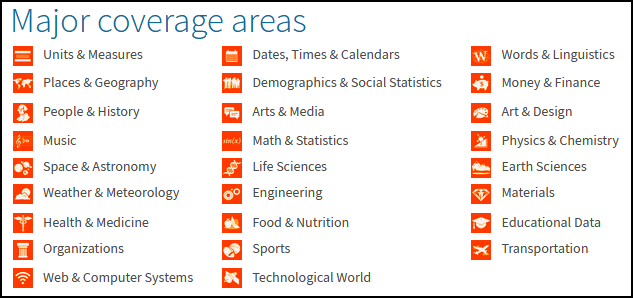
\includegraphics[scale=0.9]{images/part7/chapter_integration/integr_alg1.png}
	\caption{Рисунок. Предметные поля WDR}
	\label{fig:integr_alg1}
\end{figure}

Отметим несколько примеров. Располагая обширной статистикой по сотням тысяч учебных заведений по всему миру, \textit{Wolfram|Alpha} может вычислять ответы на сложные вопросы об образовании.
Можно запросить, какие академические степени получают студенты престижных университетов. 
Также можно рассчитать среднюю зарплату учителей в конкретном школьном округе, узнать больше о баллах обучаемых, сравнить соотношение учащихся и преподавателей в разных странах и многое другое.

\textit{\nameref{fig:integr_alg2}} иллюстрирует ответ на запрос о числе студентов в Республике Беларусь. 
\begin{figure}[H]
	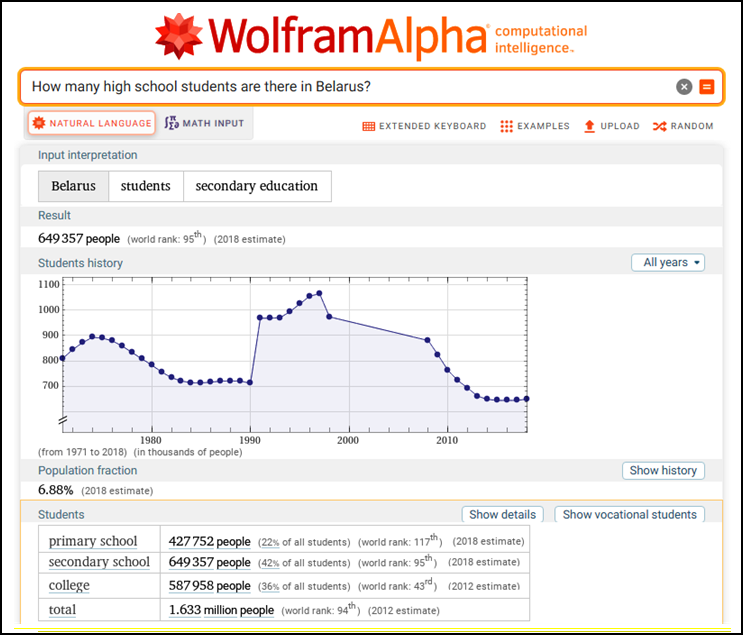
\includegraphics[scale=0.7]{images/part7/chapter_integration/integr_alg2.png}
	\caption{Рисунок. Число студентов в Республике Беларусь}
	\label{fig:integr_alg2}
\end{figure}

Сопоставление для университетов БГУ и БГУИР иллюстрирует  \textit{\nameref{fig:integr_alg3}}
\begin{figure}[H]
	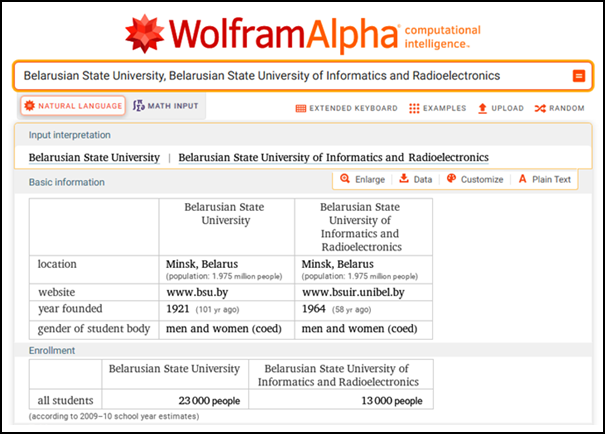
\includegraphics[scale=0.86]{images/part7/chapter_integration/integr_alg3.png}
	\caption{Рисунок. Сравнение БГУ и БГУИР}
	\label{fig:integr_alg3}
\end{figure}

\textbf{База знаний Wolfram. Представление знаний и доступ к ним.}

Доступ к базе знаний \textit{Wolfram} глубоко интегрирован в \textit{Wolfram Language}. Лингвистика свободной формы позволяет легко идентифицировать многие миллионы сущностей и многие тысячи свойств и автоматически генерировать точные представления \textit{Wolfram Language} (\textit{WL}), подходящие для обширных дальнейших вычислений. \textit{WL} также поддерживает пользовательские хранилища сущностей, которые позволяют выполнять те же вычисления, что и встроенная база знаний, и могут быть связаны с внешними реляционными \textit{базами данных}. 

Отметим основные группы функций \textit{Wolfram Mathematica} для работы с \textit{WDR}: 
\textit{Entity, EntityClass, EntityValue, Transformations, Computations on Entity Classes, Standard Properties, Specific Domains, Setting Up Custom Entity Stores, Wolfram Data Repository, Wolfram Data Drop, Setting Up Custom Entity Stores, External Knowledgebases, External Database Connectivity, Web Content, Textual Question Answering, System Configuration}. 
В каждой из перечисленных групп более трех подгрупп. Например, в группу \textit{Textual Question Answering} включены: 
\begin{textitemize}
	\item FindTextualAnswer attempt to find answers to questions from text;
	\item SemanticInterpretation convert free-form linguistics to Wolfram Language for; SemanticInterpretation["string"] attempts to give the best semantic interpretation of the specified free-form string as a Wolfram Language expression; 
	\item SemanticImport import data, converting entities etc. to Wolfram Language form, 
	\item Interpreter interpret input of various types (e.g. ``City'', ``Date'', etc.); Interpreter attempt to interpret strings of a wide variety of types; Interpreter[form] represents an interpreter object that can be applied to an input to try to interpret it as an object of the specified form.
\end{textitemize}

\textbf{Семантический анализ естественно-языковых текстов в Mathematica}. 

Люди взаимодействуют друг с другом с помощью речи и текста, и это называется \textit{естественным языком}. Компьютеры понимают естественный язык людей с помощью \textit{обработки естественного языка} (Natural Language Processing).

\textit{обработка естественного языка} --- это процесс манипулирования речью текста людьми с помощью \textit{Искусственного интеллекта}, чтобы компьютеры могли их понимать. 
Человеческий язык имеет много значений, выходящих за рамки буквального значения слов. Есть много слов, которые имеют разные значения, или любое предложение может иметь разные оттенки, такие как эмоциональный или саркастический. Компьютерам очень трудно интерпретировать значение этих предложений. 

\myuline{NLP. Основные приложения, инструменты, реализованные в системе \textit{Wolfram Mathematica} NLP}.

Ниже упомянуты, приведены несколько представительных примеров с пояснениями функций \textit{WL} групп \textit{Structural Text Manipulation}, \textit{Text Analysis}, \textit{Natural Language Processing}. 

В некотором смысле приведенные категории условны, функций и реализуемых ими возможностей много. Например, к подгруппе \textit{Structural Text Manipulation} можно отнести следующие: 
\textit{TextCases} --- \textit{extract symbolically specified elements (TextCases[text, form] gives a list of all cases of text identified as being of type form that appear in text); TextSentences --- extract a list of sentences (TextSentences["string"] gives a list of the runs of characters identified as sentences in string); TextWords --- extract a list of words (TextWords["string"] gives a list of the runs of characters identified as words in string); SequenceAlignment --- find matching sequences in text; TextStructure["text"] generates a nested collection of TextElement objects representing the grammatical structure of natural language text}.

Пример и результат выполнения функции \textit{TextStructure} к тексту \textit{``Open Semantic Technologies for Intelligent Systems''} с опцией \textit{``PartsOfSpeech''} показан на \textit{\nameref{fig:integr_alg4}}
\begin{figure}[H]
	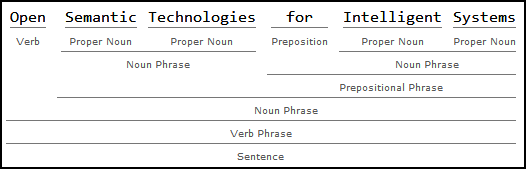
\includegraphics[scale=0.8]{images/part7/chapter_integration/integr_alg4.png}
	\caption{Рисунок. Составляющие фрагмента текста}
	\label{fig:integr_alg4}
\end{figure}

Вариант вывода с опцией \textit{``DependencyGraphs''} показан на \textit{\nameref{fig:integr_alg5}}
\begin{figure}[H]
	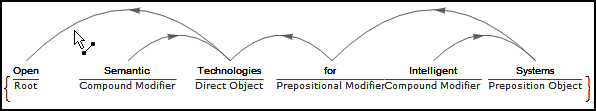
\includegraphics[scale=0.71]{images/part7/chapter_integration/integr_alg5.png}
	\caption{Рисунок. Составляющие фрагмента текста в формате DependencyGraphs}
	\label{fig:integr_alg5}
\end{figure}

\myuline{NLP. Примеры использования функции FindTextualAnswer}.

Ответы на вопросы на естественном языке из текста. Найти текстовый ответ \textit{NLP}. 
В приведенных ниже двух примерах объектом обработки является текст \textit{``International scientific and technical conference proceedings Open Semantic Technologies for Intelligent Systems (OSTIS). Established: 2011. Scientific areas of the conference: 05.13.11, 05.13.15, 05.13.17''}.

В варианте запроса с опцией \textit{``Date of establishment of the conference?''} ответом является
\begin{center}
	\fbox{\textit{``2011''}}
\end{center}
В варианте запроса с опциями \textit{``Date of establishment of the conference?''}, ``Scientific \textit{areas of the conference?''} ответом является список 
\begin{center}
	\fbox{\textit{``2011'', ``05.13.11, 05.13.15, 05.13.17''}}
\end{center}

\myuline{Примеры извлечения знаний, сущности или темы из статей Википедии}.

Данные \textit{Википедии} используют \textit{программный интерфейс} \textit{MediaWiki} для извлечения содержимого статей и категорий, а также метаданных из \textit{Википедии}. Статья может быть указана, как строка или объект языка \textit{Wolfram}. 
Извлечение статей, ассоциированных с сущностями языка, обеспечивает функция \textit{Wolfram Mathematica} \textit{TextSentences}, в частности, можно работать с ресурсами \textit{Википедии}. 
Ниже на \textit{\nameref{fig:integr_alg6}} представлен результат выполнения функции \textit{TextSentences}, с параметрами \textit{WikipediaData}, \textit{Entity}, \textit{``Person''}, \textit{``AlexeiLeonov''}.
 
\begin{figure}[H]
	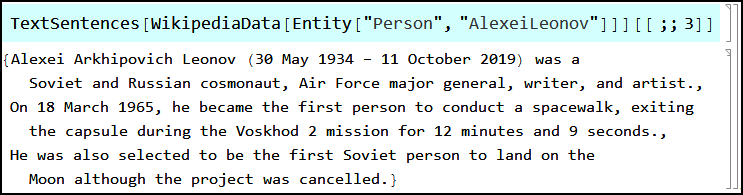
\includegraphics[scale=0.55]{images/part7/chapter_integration/integr_alg6.png}
	\caption{Рисунок. Сведения из Wikipedia о космонавте Leonov}
	\label{fig:integr_alg6}
\end{figure}

\textit{\nameref{fig:integr_alg7}} иллюстрирует ответ системы на выполнение функции \textit{WikipediaData} с параметрами \textit{``Voskhod 2''}, \textit{``ImageList''}.

\begin{figure}[H]
	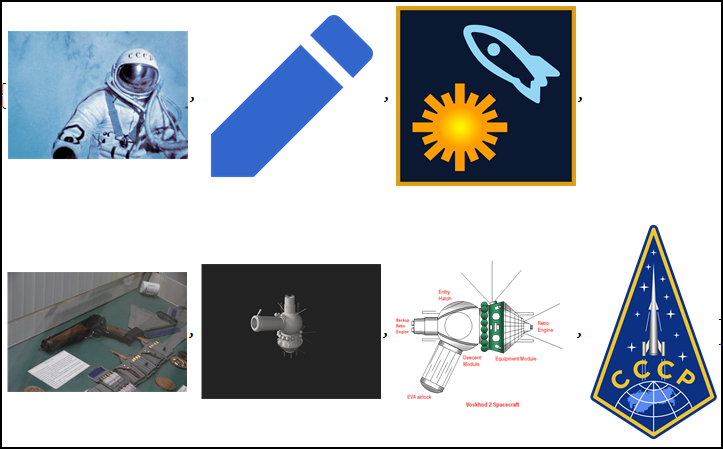
\includegraphics[scale=0.56]{images/part7/chapter_integration/integr_alg7.png}
	\caption{Выборка в Wikipedia иллюстраций по Voskhod 2}
	\label{fig:integr_alg7}
\end{figure}

Приведенные примеры работы с базами знаний средствами \textit{Wolfram Mathematica}, так как функции ядра системы можно использовать в разработанных на других платформах программах, можно трактовать, как предложения инновационного совершенствования имеющихся инструментальных средств, компонентов любых интеллектуальных компьютерных систем, и конечно же \textit{Экосистемы OSTIS}.

\subsection{Пример интеграции прототипа обучающей ostis-системы по дискретной математике и Wolfram Mathematica}.
\label{subsec_cas_intergation}

Приведем иллюстрации совместного использования при работе с графами прототипа обучающей \textit{ostis-системы} по дискретной математике, входящей в состав \textit{Экосистемы OSTIS}, и \textit{Wolfram Mathematica}. Отмеченные ниже результаты показывают возможности использования в ostis-системе выполняемых в \textit{Wolfram Mathematica} результатов расчетов и визуализации. Причем, реализации доступны с использованием соответствующего программного интерфейса (можно выполнить размещенный в облаке Wolfram код на Wolfram Language в рамках пользовательской программы, например, на \textit{Python} или \textit{C++} --- https://reference.wolfram.com/language/ref/APIFunction.html]) или средств импорта, экспорта. 

Отдельно отметим, какие форматы поддерживаются системой \textit{Wolfram Mathematica}. Согласно системной функции \textit{Mathematica} \myuline{\$ImportFormats}, имеем следующий перечень:
\textit{3DS, ACO, Affymetrix, AgilentMicroarray, AIFF, ApacheLog, ArcGRID, AU, AVI, Base64, BDF, Binary, Bit, BMP, BSON, Byte, BYU, BZIP2, CDED, CDF, Character16, Character8, CIF, Complex128, Complex256, Complex64, CSV, CUR, DAE, DBF, DICOM, DIF, DIMACS, Directory, DOT, DXF, EDF, EML, EPS, ExpressionJSON, ExpressionML, FASTA, FASTQ, FCS, FITS, FLAC, GenBank, GeoJSON, GeoTIFF, GIF, GPX, Graph6, Graphlet, GraphML, GRIB, GTOPO30, GXL, GZIP, HarwellBoeing, HDF, HDF5, HIN, HTML, HTTPRequest, HTTPResponse, ICC, ICNS, ICO, ICS, Ini, Integer128, Integer16, Integer24, Integer32, Integer64, Integer8, JavaProperties, JavaScriptExpression, JCAMP-DX, JPEG, JPEG2000, JSON, JVX, KML, LaTeX, LEDA, List, LWO, M4A, MAT, MathML, MBOX, MCTT, MDB, MESH, MGF, MIDI, MMCIF, MO, MOL, MOL2, MP3, MPS, MTP, MTX, MX, MXNet, NASACDF, NB, NDK, NetCDF, NEXUS, NOFF, OBJ, ODS, OFF, OGG, OpenEXR, Package, Pajek, PBM, PCAP, PCX, PDB, PDF, PGM, PHPIni, PLY, PNG, PNM, PPM, PXR, PythonExpression, QuickTime, Raw, RawBitmap, RawJSON, Real128, Real32, Real64, RIB, RLE, RSS, RTF, SCT, SDF, SDTS, SDTSDEM, SFF, SHP, SMA, SME, SMILES, SND, SP3, Sparse6, STL, String, SurferGrid, SXC, Table, TAR, TerminatedString, TeX, Text, TGA, TGF, TIFF, TIGER, TLE, TSV, UBJSON, UnsignedInteger128, UnsignedInteger16, UnsignedInteger24, UnsignedInteger32, UnsignedInteger64, UnsignedInteger8, USGSDEM, UUE, VCF, VCS, VTK, WARC, WAV, Wave64, WDX, WebP, WLNet, Wolfram MathematicaLF, WXF, XBM, XHTML, XHTMLMathML, XLS, XLSX, XML, XPORT, XYZ, ZIP.}

В рассматриваемом ниже примере исходные данные (некоторый конкретный граф) поступают (выполняется импорт) из обучающей \textit{ostis-системы по дискретной математике}, визуализируются средствами графики \textit{Wolfram Mathematica}, затем осуществляется решение типичной задачи и предпочтительные итоговые результаты экспортируются обратно в обучающую \textit{ostis-систему} по дискретной математике. Исходные данные к задаче, используемый далее конкретный граф показан на \textit{\nameref{fig:integr_alg31}}:

%TODO Нарисовать в SCg

\begin{figure}[H]
	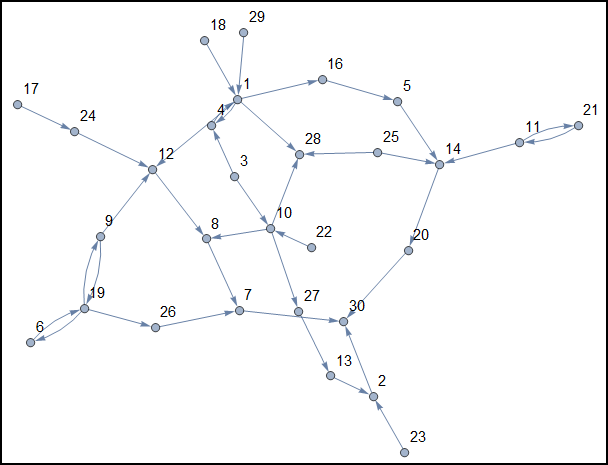
\includegraphics[scale=0.9]{images/part7/chapter_integration/integr_alg31.png}
	\caption{Рисунок. Используемый далее граф, вершины и дуги (отображение в  ostis-системе)}
	\label{fig:integr_alg31}
\end{figure}

Следующие иллюстрации получены в \textit{Wolfram Mathematica}. 

Для импортированного графа в \textit{Wolfram Mathematica} можно получить общую информацию, например: число вершин, дуг, список ребер (напомним, что граф выше сформирован в обучающей \textit{ostis-системе} по дискретной математике), визуализировать уже в \textit{Wolfram Mathematica}. На \textit{\nameref{fig:integr_alg31d}}
показаны результаты вывода в \textit{Wolfram Mathematica} списка вершин (VertexList), числа дуг (EdgeCount), дуги (EdgeList):
\begin{figure}[H]
	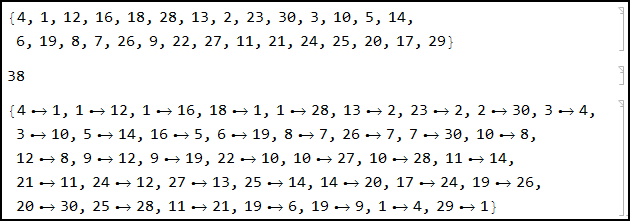
\includegraphics[scale=0.65]{images/part7/chapter_integration/integr_alg31d.png}
	\caption{Рисунок. Используемый граф, общая информация (вывод в Wolfram Mathematica)}
	\label{fig:integr_alg31d}
\end{figure}

Для примера визуализации ниже показаны 3 варианта вывода. На \textit{\nameref{fig:integr_alg32}} приведены связи с указанием направлений:
\begin{figure}[H]
	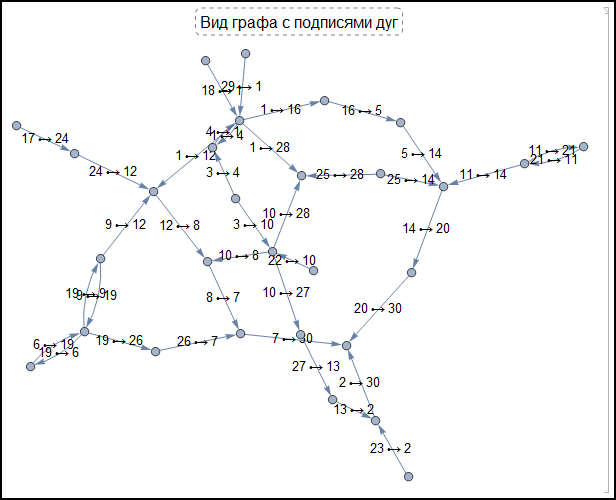
\includegraphics[scale=0.68]{images/part7/chapter_integration/integr_alg32.png}
	\caption{Рисунок. Используемый граф, дуги (вывод в Wolfram Mathematica)}
	\label{fig:integr_alg32}
\end{figure}

Вывод на \textit{\nameref{fig:integr_alg33}} реализован с указанием стилей вершин и их номеров, задано, что все дуги от узла с большим номером к узлу с меньшим выводятся пунктирными красными линиями, а остальные сплошными зелеными:

\begin{figure}[H]
	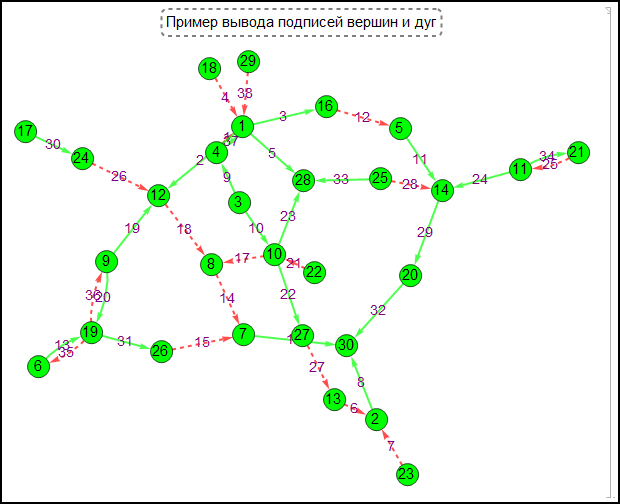
\includegraphics[scale=0.88]{images/part7/chapter_integration/integr_alg33.png}
	\caption{Рисунок. Используемый граф с оформлением по правилам (вывод в Wolfram Mathematica)}
	\label{fig:integr_alg33}
\end{figure}

Пример вывода с заданием формата укладки графа DiscreteSpiralEmbedding, применения опций оформления вершин реализован при выводе на \textit{\nameref{fig:integr_alg34}} 

\begin{figure}[H]
	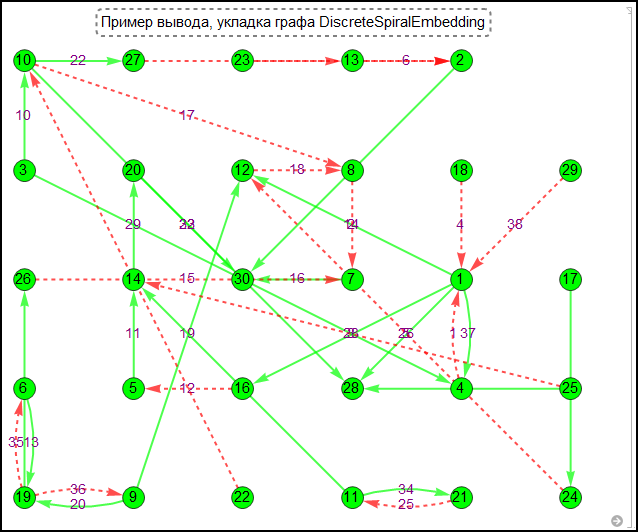
\includegraphics[scale=0.87]{images/part7/chapter_integration/integr_alg34.png}
	\caption{Рисунок. Используемый граф с оформлением DiscreteSpiralEmbedding (вывод в Wolfram Mathematica)}
	\label{fig:integr_alg34}
\end{figure}

Пример решения задачи нахождения кратчайшего пути между двумя вершинами иллюстрирует \textit{\nameref{fig:integr_alg34}}. (При решении использованы функции \textit{Wolfram Mathematica}: GraphDistance, NeighborhoodGraph, Sow, DirectedEdge, Placed, Union, Flatten).

\begin{figure}[H]
	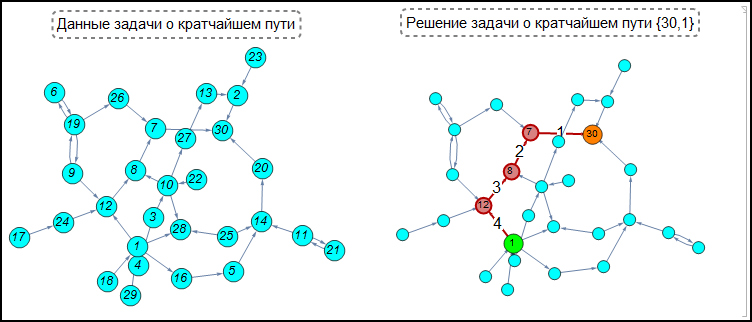
\includegraphics[scale=0.55]{images/part7/chapter_integration/integr_alg35.png}
	\caption{Рисунок. Решение задачи нахождения кратчайшего пути между двумя вершинами (вывод в Wolfram Mathematica)}
	\label{fig:integr_alg35}
\end{figure}

Полученные и рассмотренные результаты включают трудоемкие для реализации на языках программирования задачи графики, а также математически и алгоритмически сложные задачи предметной области. Представленные варианты визуализации, нахождения решения требуют только внимательного изучения примеров системы помощи \textit{Wolfram Mathematica}, определенных навыков программирования, т.е. доступны большинству инженеров-программистов. Перенести результаты в другие программные приложения также не сложно, потому что \textit{Wolfram Mathematica} предоставляет возможности экспорта в любые типовые форматы.

\subsection*{Заключение к \ref{sec_integration_algebra}}

Системы компьютерной алгебры на настоящий момент представляют собой мощные инструментальные комплексы, возможности которых давно вышли за рамки алгебраических вычислений и даже классической математики в целом. Лидеры \textit{с.к.а.} предоставляют множество возможностей вычислений, алгоритмов обработки, анализа, визуализации. Одним из лидеров является система \textit{Wolfram Mathematica}, ядро которой содержит более 6000 функций. Компанией \textit{Wolfram} также разработаны много уникальных проектов, в число которых кроме системы \textit{Wolfram Mathematica} входит вопросно-ответная система \textit{Wolfram Alpha} (см. \scncite{WolframAlpha}), содержащая обширную базу знаний и набор вычислительных алгоритмов. 

В основе представления фактографических, логических и процедурных знаний для систем семейства \textit{Wolfram} лежит мультипарадигмальный язык программирования \textit{Wolfram Language}. Наличие такого внутреннего языка описания функций систем \textit{Wolfram} и в целом высокий уровень документированности этих функций выгодно отличает системы \textit{Wolfram} от других сервисов, позволяющих решать общие и частные задачи. Отличие заключается в том, что во многих случаях система семейства \textit{Wolfram} может не просто решить задачу, но и \myuline{объяснить} ход решения, а также помочь пользователю в выборе той или иной функции, подходящей для решения его задачи, или предложить набор функций, которые можно применить к данным, полученным в результате решения исходной задачи. Другим достоинством систем семейства \textit{Wolfram} является им комплексность, позволяющая решать достаточно сложные задачи в рамках одного приложения и без необходимости интеграции разнородных сервисов.

Учитывая перечисленное, можно сделать вывод о целесообразности интеграции системы компьютерной алгебры \textit{Wolfram Mathematica} с \textit{ostis-системами}, входящими в состав \textit{Экосистемы OSTIS}. В параграфе были рассмотрены возможные принципы такой интеграции и показаны соответствующие примеры.

%\input{author/references}
\section*{Заключение к Главе \ref{chapter_integration}}

При \textit{интеграции} различных \textit{сервисов} и \textit{информационных ресурсов} с \textit{Экосистемой OSTIS} пользователь может получить ряд значительных преимуществ, которые могут повысить эффективность его деятельности:
\begin{textitemize}
	\item повышение точности и качества данных, получение более точной и полной информации, что может повысить качество принимаемых решений (это особенно важно в условиях быстро меняющейся среды, когда точность и качество данных играют решающую роль);
	\item улучшение управления и контроля процессов обмена информацией, что может помочь в принятии быстрых и правильных решений;
	\item снижение затрат на разработку и поддержку приложений, улучшение скорости разработки новых приложений, а также повышение качества их реализации (это связано с тем, что \textit{Экосистема OSTIS} позволяет использовать уже существующие компоненты, что сокращает время и затраты на разработку).
\end{textitemize}
